\documentclass[a4paper,12pt]{report}

\usepackage{alltt, fancyvrb, url}
\usepackage{graphicx}
\usepackage[utf8]{inputenc}
\usepackage{float}
\usepackage{xcolor}
\usepackage{hyperref}

% Questo commentalo se vuoi scrivere in inglese.
\usepackage[italian]{babel}

\usepackage[italian]{cleveref}

\title{Relazione Temple-Tower per\\``Programmazione ad Oggetti''}

\author{Davide Vignali, Marko Cobo, Mattia Mularoni, Nicolas Montanari}
\date{\today}


\begin{document}

\maketitle

\tableofcontents

\chapter{Analisi}

\section{Descrizione e requisiti}

Il progetto Temple Tower si ispira ai classici dungeon crawler, offrendo un’esperienza di gioco a livelli in cui il giocatore esplora piani di un dungeon circolare per raccogliere tesori, sconfiggere nemici e salire verso il livello successivo. Il gioco culmina in un epico scontro con un boss finale.
%
La meccanica dei livelli circolari prende ispirazione dal gioco \href{https://ring-of-pain.fandom.com/wiki/Ring_of_Pain_Wiki}{Ring of Pain}.


\subsection*{Requisiti funzionali}
\begin{itemize}
	\item L'area di gioco è circolare ed è composta da diverse caselle contententi gli elementi di gioco che possono essere positivi o negativi per il giocatore.
	\item Gli elementi di gioco sono rappresentati da tesori (possono contenere punti esperienza, armi), trappole (tolgono punti vita), scale (permettono il passaggio a un livello superiore).
	\item Il giocatore si può muovere all'interno del livello, può combattere contro i nemici,  interagire con gli elementi di gioco.
	\item Dopo ogni scontro con un nemico o dopo aver attraversato una trappola il giocatore perde i punti vita, al termine dei quali la partita termina e si ritorna alla schermata inziale.
    \item Generazione casuale della torre per permettere partite sempre diverse.
\end{itemize}

\subsection*{Requisiti non funzionali}
\begin{itemize}
	\item Una volta arrivato all'ultimo piano il giocatore incontrerà il boss finale, il quale avrà comportamenti  unici e una difficoltà maggiore rispetto ai nemici normali .
	\item Difficoltà variabile in base al progresso di gioco.
	\item Musica di sottofondo e feedback sonori associati alle varie azioni.
	\item Esistono più tipologie di armi la quale efficacia varia rispetto al tipo di nemico.
\end{itemize}

\section{Modello del Dominio}
\textbf{Temple Tower} sarà rappresentato da una torre composta da un certo numero di piani (\textit{Floor}), 
%
ciascuno dei quali conterrà stanze collegate tra loro. Ogni stanza potrà contenere una trappola, un nemico, un tesoro e ospitare il giocatore.

\begin{itemize}
    \item \textbf{Trappole}: infliggono danni al giocatore.
    \item \textbf{Nemici}: attaccano il giocatore in combattimenti a turni.
    \item \textbf{Tesori}: forniscono punti vita, nuove armi, oppure potrebbe essere una trappola.
\end{itemize}
%
Il giocatore potrà utilizzare armi per affrontare i nemici. Poiché gli attacchi avvengono a turni, 
%
sarà fondamentale bilanciare le statistiche per evitare vittorie "matematiche" dovute a differenze di efficacia delle armi. 
%
Il giocatore e i nemici avranno a disposizione diverse tipologie di mosse di attacco e armi, che possono variare in potenza ed effetto.
%
Dopo aver esplorato le stanze di un piano, il giocatore potrà utilizzare le scale per salire al piano successivo della torre. 
%
Durante la partita, sia il giocatore sia i nemici avranno delle barre di stato: \textbf{vita}.
%
\begin{itemize}
    \item \textbf{Barra della vita}: si riduce subendo danni da nemici o trappole. Quando arriva a zero, la partita termina e si ricomincia dall'inizio.
\end{itemize}
%
All’ultimo piano, il giocatore affronterà il \textbf{boss finale}, un nemico più forte, dotato di mosse di attacco avanzate e particolari rispetto ai nemici ordinari.
%
Per arricchire l’esperienza, sarà presente un sottofondo musicale durante tutto il gioco.
%
\begin{figure}[H]
	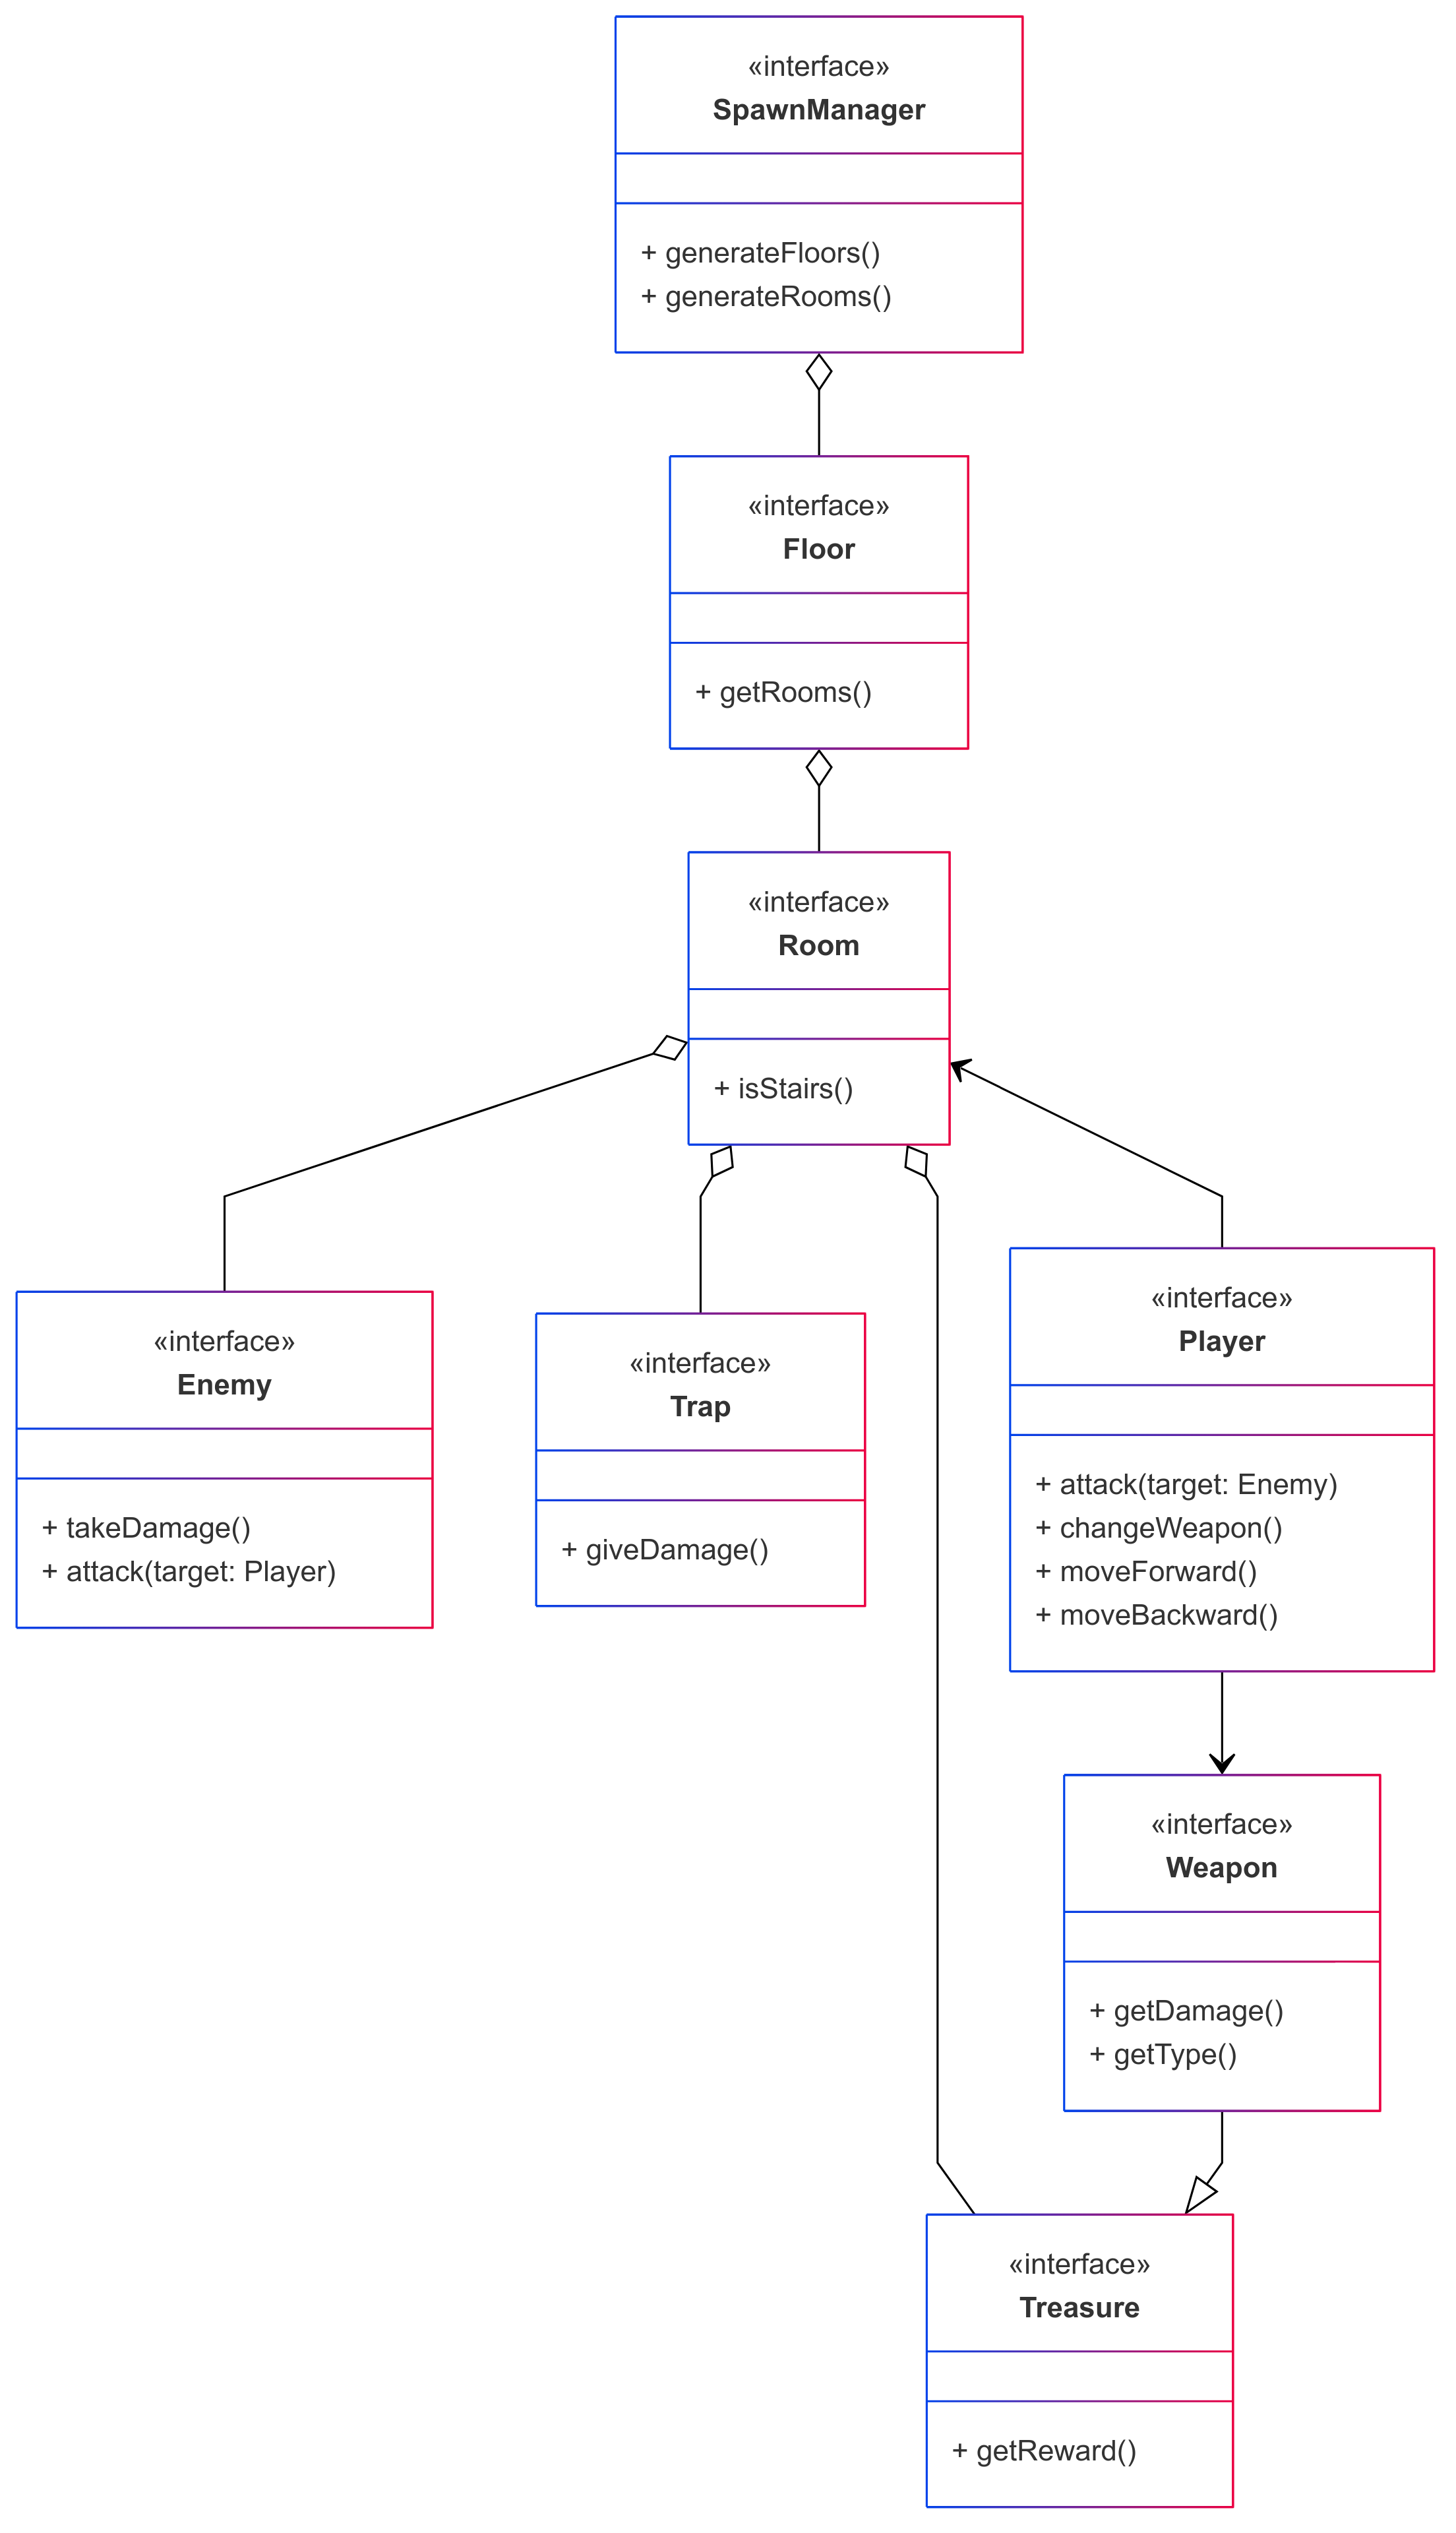
\includegraphics[scale=0.15]{img/analisys.png}
\end{figure}

\chapter{Design}

\section{Architettura}

L'architettura del gioco \textbf{Temple Tower} segue il pattern architetturale \textbf{Model-View-Controller (MVC)} per garantire una chiara separazione delle responsabilità tra la logica di business, la presentazione e la gestione degli eventi.

\subsection*{Composizione del Pattern MVC}
\begin{itemize}
    \item \textbf{Model}: 
    \begin{itemize}
        \item Rappresenta la logica principale del gioco e include classi come \texttt{Tower}, \texttt{Floor}, \texttt{RoomBehavior}, \texttt{Player}, e i vari tipi di stanze (\texttt{EnemyRoom}, \texttt{TreasureRoom}, \texttt{StairsRoom}) che implementano il pattern Strategy.
        \item Questo approccio consente di definire comportamenti specifici per ogni tipologia di stanza in modo modulare, rendendo semplice l'aggiunta di nuovi tipi di stanze senza modificare il codice esistente.
        \item La logica di gioco, come il movimento del giocatore o gli effetti delle interazioni con nemici, trappole o tesori, è interamente contenuta nel model.
    \end{itemize}

    \item \textbf{View}: 
    \begin{itemize}
        \item Tutta la view è gestita da uno (\texttt{SceneManager}), il quale si occupa, mediante l'implementazione di un pattern Factory, di gestire il
        %
		cambiamento della vista in base alla situazione attuale.
        \item Grazie al manager è possibile decentralizzare le responsabilità della vista a n classi, le quali si occuperanno della gestione degli eventi
        %
		della singola interfaccia.
    \end{itemize}

    \item \textbf{Controller}: 
    \begin{itemize}
        \item La classe \texttt{GameController} funge da intermediario tra il modello e la vista, orchestrando il flusso degli eventi nel gioco.
        \item Gestisce le azioni dell'utente, permette al giocatore di muoversi tra le stanze (\texttt{changeRoom}) o salire al piano successivo (\texttt{gotoNextFloor}), si occupa inoltre di iniziare e terminare il gioco.
    \end{itemize}
\end{itemize} 

\subsection*{Scalabilità e Manutenibilità}
Grazie all'uso combinato dei pattern MVC e Strategy:
\begin{itemize}
    \item \textbf{Aggiunta di nuove stanze}: È possibile introdurre nuove tipologie di stanze semplicemente aggiungendo nuove implementazioni dell'interfaccia \texttt{RoomBehavior}, senza modificare altre parti del codice.
    \item \textbf{Separazione delle responsabilità}: La gestione della logica di gioco, della presentazione grafica e delle interazioni dell'utente è ben separata, favorendo la manutenibilità e la possibilità di cambiare singole componenti senza influenzare le altre.
\end{itemize}

Questa architettura rende il sistema flessibile, modulare e facilmente estensibile, adattandosi alle necessità di futuri miglioramenti o aggiunte.
%
\begin{figure}[H]
	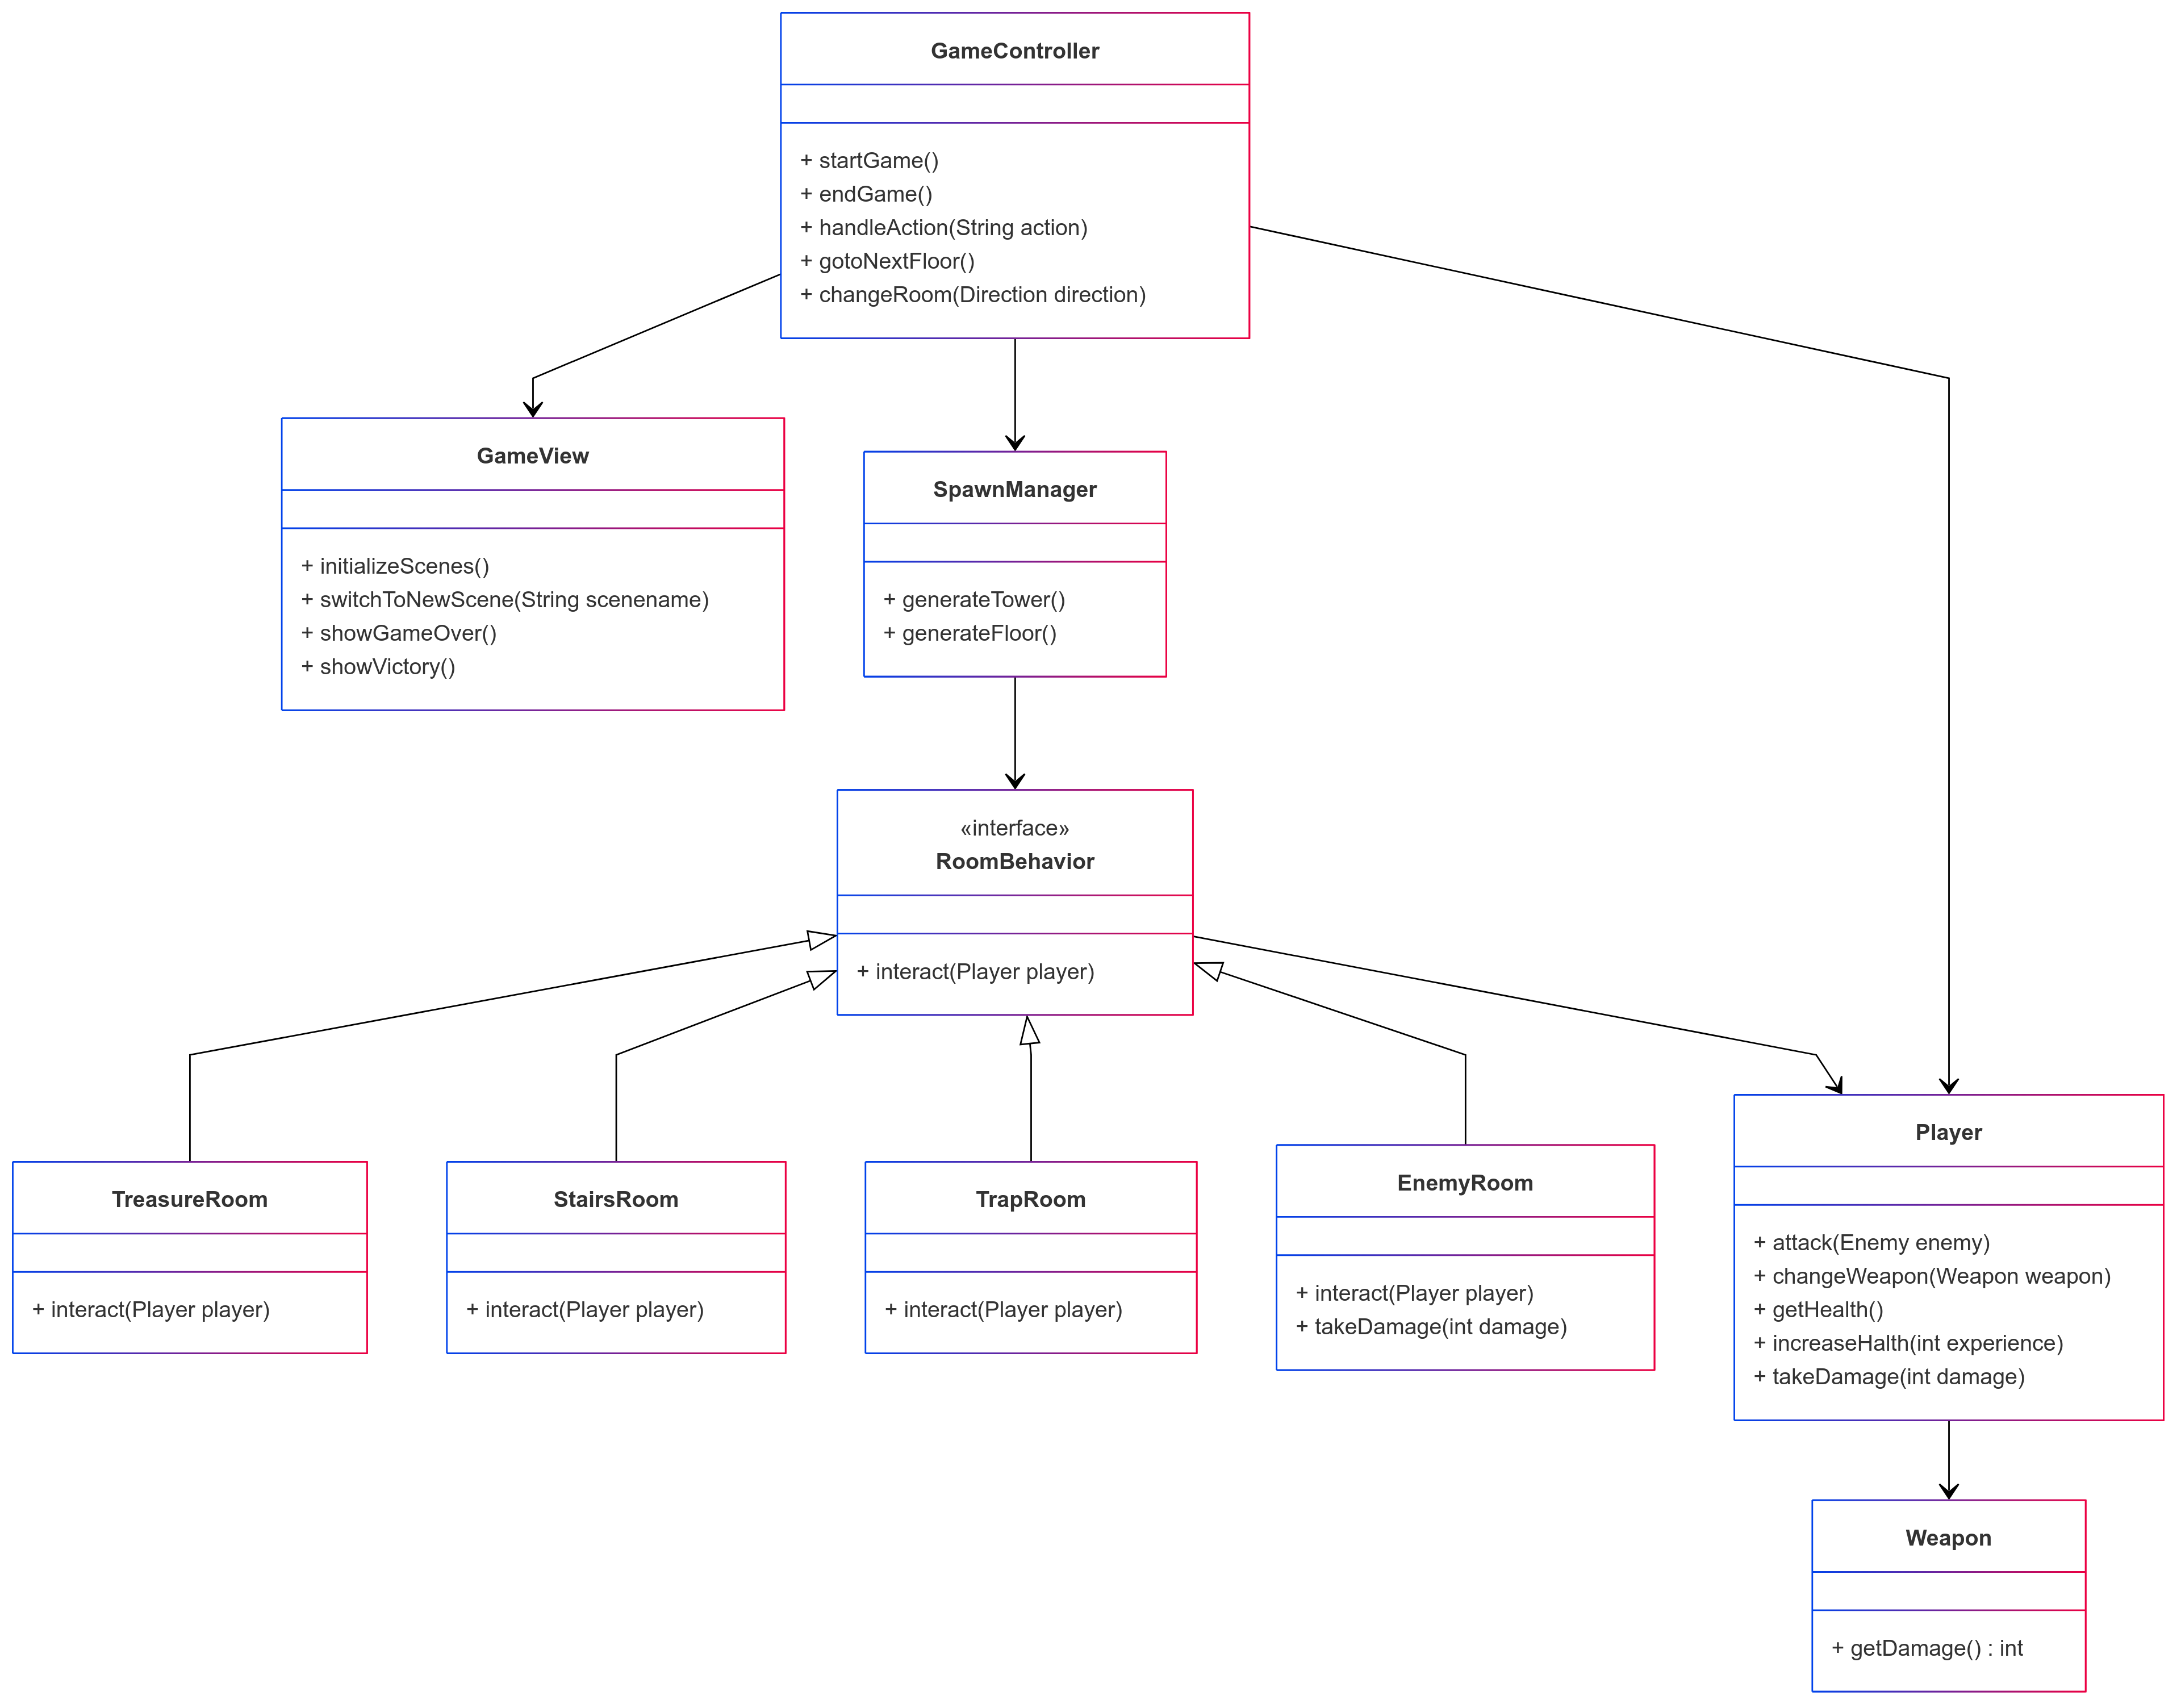
\includegraphics[scale=0.12]{img/design.png}
\end{figure}

\section{Design dettagliato}
\subsection{Cobo}
\subsubsection{Sistema di Gestione Audio}
Il sistema richiede una gestione per la riproduzione della musica di sottofondo, le cui funzionalit\`a principali sono:
\begin{itemize}
    \item Gestione del volume;
    \item Controllo dello stato di riproduzione della musica;
    \item Corretto caricamento e gestione delle risorse audio;
    \item Mantenimento di una corretta separazione tra logica, controllo e view.
\end{itemize}

\textbf {Architettura MVC}\newline
La soluzione proposta implementa un pattern Model-View-Controller (MVC) con le seguenti componenti:
\begin{itemize}
    \item \textbf{Model (MusicModel)}: Mantiene informazioni sul volume e sullo stato di riproduzione, gestisce il ciclo di vita del clip audio e lo stato interno del sistema audio.
    \item \textbf{Controller (MusicController)}: Gestisce le operazioni sulla riproduzione musicale e fa da intermediario tra View e Model.
    \item \textbf{View}: Richiama i metodi del controller per gestire la riproduzione.
\end{itemize}

\textbf{Vantaggi e svantaggi}\newline
\textbf{Pro}: Separazione delle responsabilit\`a, il MusicModel gestisce i dettagli tecnici mentre il MusicController gestisce il flusso principale.

\textbf{Contro}: Richiede una buona coordinazione tra le classi.

\textbf{Diagramma UML}\newline
\begin{figure}[h]
    \centering 
    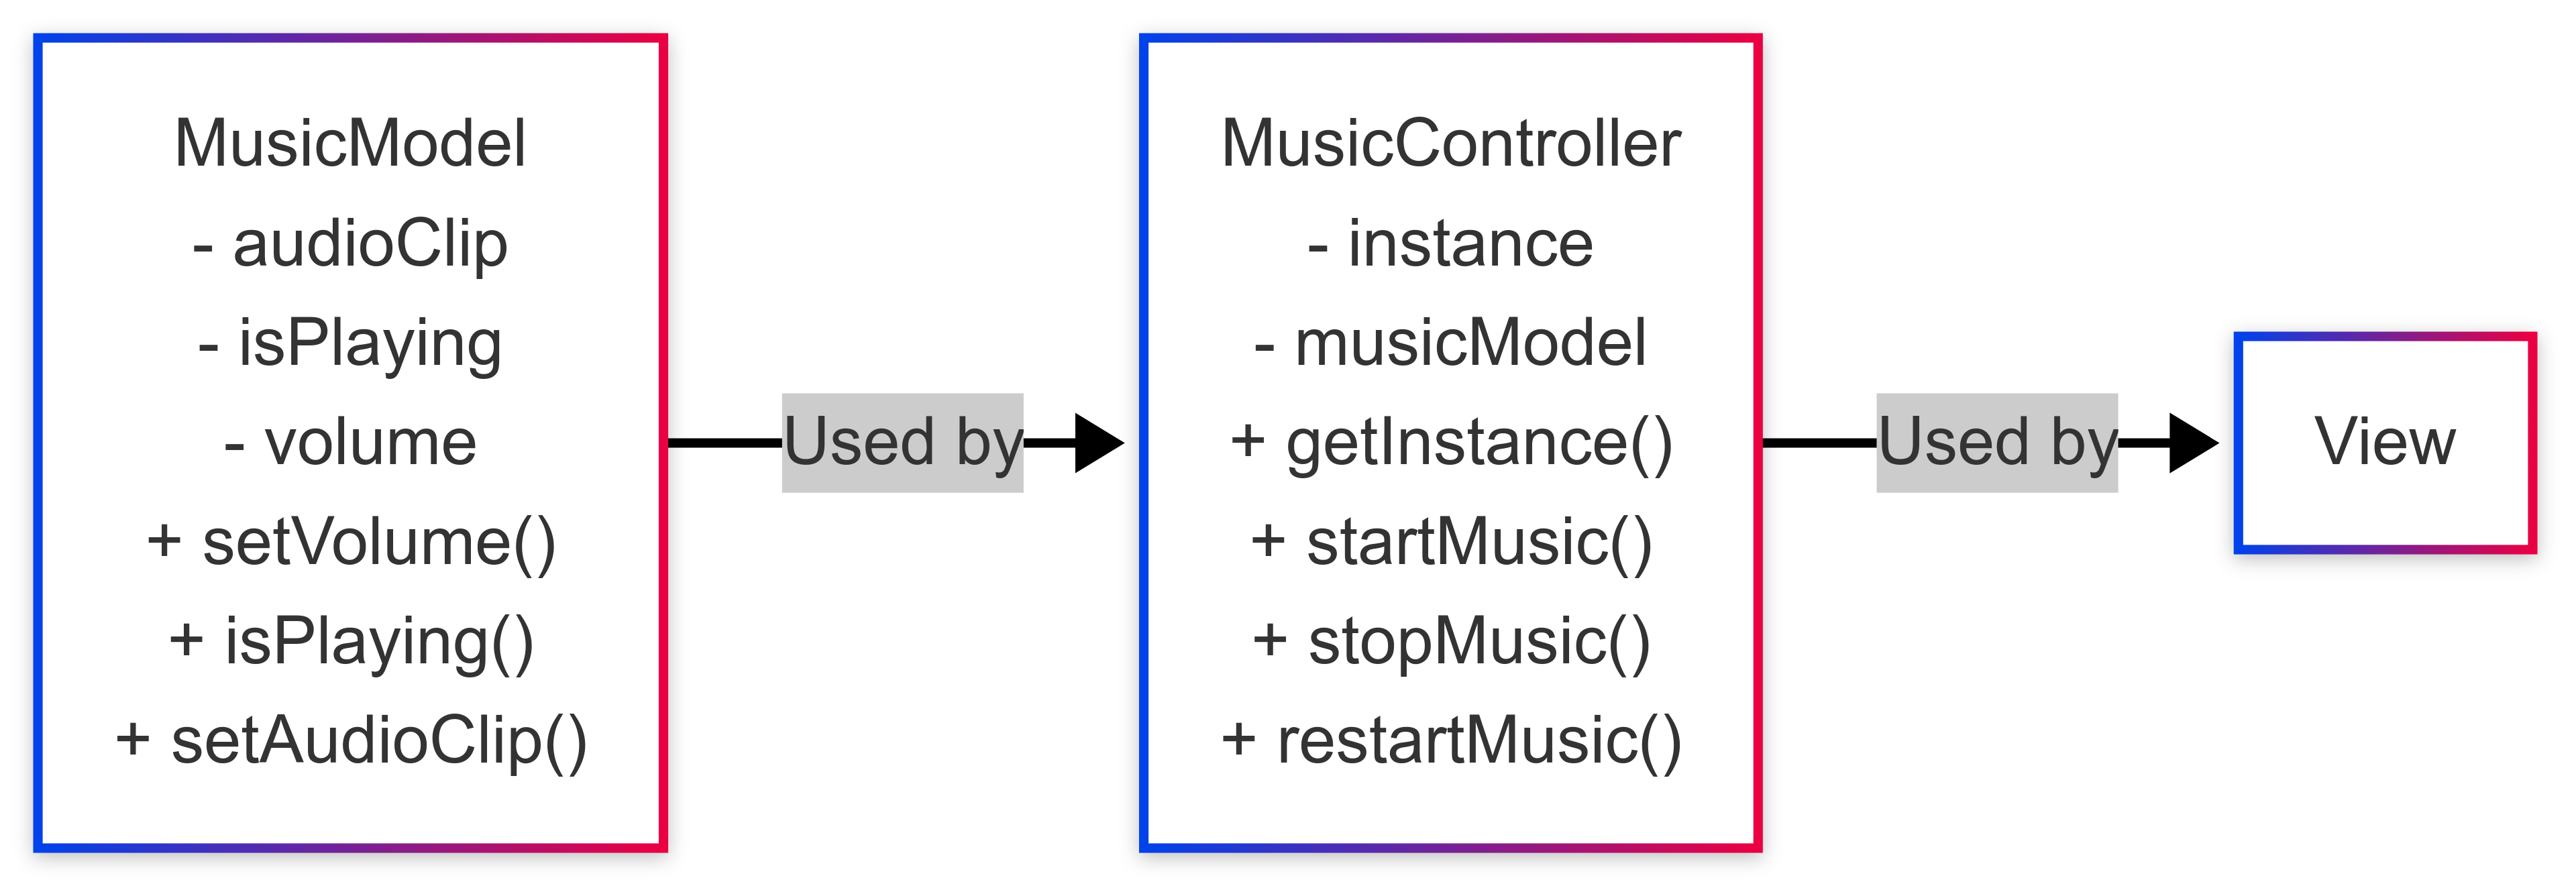
\includegraphics[width=0.8\textwidth]{img/uml_diagram.png}
    \caption{Diagramma UML del sistema di gestione audio}
    \label{fig:uml}
\end{figure}

\subsubsection{Pattern Singleton}
Il pattern Singleton \`e stato utilizzato nella classe \texttt{MusicController} per garantire che esista solo un'istanza del controller musicale durante l'intera esecuzione dell'applicazione. Questo evita conflitti e garantisce un punto di accesso globale alla gestione della musica.

\subsubsection{Metodo Template: getInstance()}
\textbf{Motivazione}: Assicura che esista solo un'istanza di \texttt{MusicController}, facilitando la gestione centralizzata della riproduzione musicale. Il pattern Singleton \`e stato utilizzato in modo appropriato per il \texttt{MusicController}, poich\'e la gestione centralizzata della riproduzione musicale richiede una singola istanza.


\subsection{Montanari}
\subsubsection{Gestione dei Popup tramite Factory Method}

\textbf{Problema}\
Nel gioco, esistono diversi tipi di finestre di dialogo (popup) che vengono mostrate in varie situazioni, come la raccolta di un'arma o il guadagno di esperienza. La creazione manuale di questi popup in ogni punto del codice porta a una duplicazione del codice e a una ridotta manutenibilit`a. Inoltre, senza un’astrazione adeguata, ogni nuova finestra di dialogo richiederebbe la scrittura ripetitiva della sua struttura, aumentando il rischio di incoerenze nel comportamento.

\textbf{Soluzione}\
Per risolvere questo problema, `e stato adottato il Factory Method, che consente di delegare la creazione dei popup a una classe centralizzata (\texttt{DialogFactory}). Questa classe definisce un metodo \texttt{createDialog} che, in base al tipo di popup richiesto, restituisce un oggetto \texttt{Dialog} con il contenuto e il comportamento appropriati.

Questa soluzione offre diversi vantaggi:
\begin{itemize}
\item \textbf{Miglior riuso del codice}: la logica di costruzione dei popup `e riutilizzabile e centralizzata.
\item \textbf{Maggiore manutenibilit`a}: per aggiungere nuovi tipi di popup, basta estendere il metodo \texttt{createDialog} senza modificare il codice esistente.
\item \textbf{Maggiore coerenza}: tutti i popup rispettano uno stile uniforme e una gestione degli eventi standardizzata.
\end{itemize}

Un’alternativa considerata era l’uso di una classe \texttt{DialogUtil} con metodi statici per ogni tipo di popup. Tuttavia, questo approccio avrebbe reso pi`u difficile estendere il sistema senza modificare direttamente la classe di utilit`a, violando il principio Open/Closed.

\textbf{Schema UML}\
Lo schema seguente mostra l'implementazione del Factory Method per la creazione dei popup:

\begin{figure}[H]
	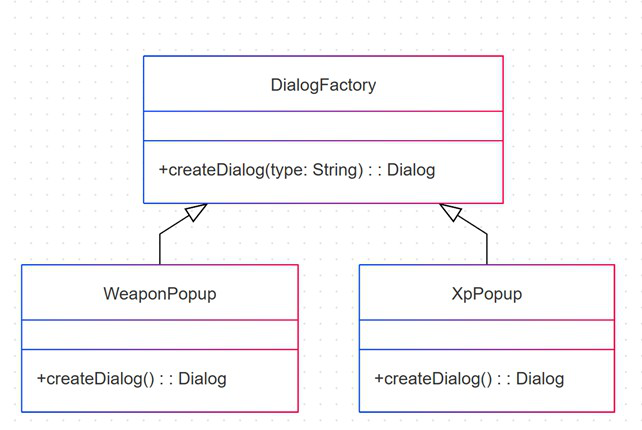
\includegraphics[scale=0.8]{img/montanariDialog.png}
\end{figure}

\textbf{Applicazione del Pattern Factory Method}\
\begin{itemize}
\item \texttt{DialogFactory} `e la classe che definisce il metodo \texttt{createDialog}, delegando la creazione alle classi specifiche.
\item \texttt{WeaponPopup} e \texttt{XpPopup} sono le sottoclassi che sovrascrivono il metodo factory per fornire l’implementazione specifica del popup.
\item Il codice client utilizza \texttt{DialogFactory.createDialog()} per ottenere il popup corretto senza conoscere i dettagli della sua implementazione.
\end{itemize}

Questa implementazione segue il pattern Factory Method, migliorando la separazione delle responsabilit`a e facilitando l’aggiunta di nuovi tipi di popup in futuro.

\subsubsection{Gestione della Sincronizzazione tra Attacco, Punti Vita e UI}

\textbf{Problema}
Nel contesto della gestione della scena di combattimento, è emersa la necessità di garantire una sincronizzazione corretta tra l'attacco del giocatore, la riduzione dei punti vita dell'avversario e l'aggiornamento dell'interfaccia utente (UI). Un’errata gestione di questo processo potrebbe causare incongruenze visive o problemi di gameplay, come:
\begin{itemize}
    \item Attacchi non registrati;
    \item Aggiornamenti tardivi della UI;
    \item Reazioni non coerenti tra azione e conseguenza.
\end{itemize}

\textbf{Soluzione}
Per affrontare questa problematica, è stata implementata una gestione sequenziale delle azioni attraverso l'uso combinato di:
\begin{itemize}
    \item \textbf{Animazioni} (\texttt{Timeline}) per gestire i movimenti visivi;
    \item \textbf{Ritardi programmati} (\texttt{PauseTransition}) per sincronizzare le azioni;
    \item \textbf{Aggiornamenti sincroni della UI} (\texttt{Platform.runLater}) per garantire modifiche sicure nel thread principale.
\end{itemize}

Il flusso di esecuzione prevede i seguenti passaggi:
\begin{enumerate}
    \item L’attacco viene eseguito, attivando un'animazione di avanzamento del giocatore o un effetto visivo (ad esempio, una fiamma).
    \item Una volta terminata l’animazione, il danno viene applicato riducendo i punti vita dell’avversario.
    \item La UI viene aggiornata, modificando la barra della salute (\texttt{ProgressBar}) e il valore numerico degli HP dell'avversario.
    \item Se il nemico è ancora in vita, viene avviato un ritardo tramite \texttt{PauseTransition}, che simula il tempo di reazione prima della sua risposta.
    \item Il nemico esegue il contrattacco, aggiornando la UI con la nuova quantità di punti vita del giocatore.
    \item Si verifica se il combattimento è terminato:
    \begin{itemize}
        \item In caso di vittoria del giocatore, il pulsante di attacco viene disabilitato e la salute viene ripristinata.
        \item In caso di sconfitta, viene mostrato un popup che reindirizza il giocatore al menu principale.
    \end{itemize}
\end{enumerate}

\textbf{Schema UML}\
Lo schema seguente mostra l'implementazione di una parte delle classi utilizzate

\begin{figure}[H]
	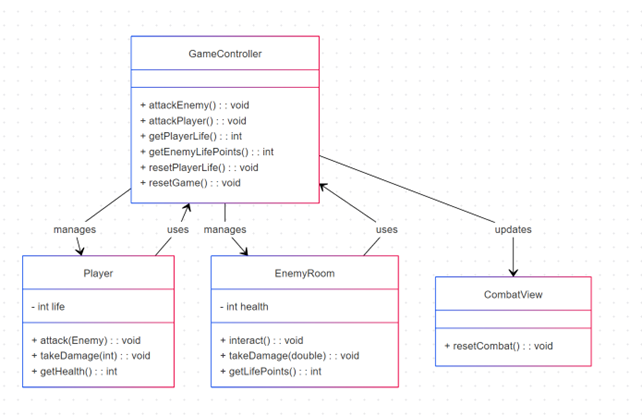
\includegraphics[scale=0.9]{img/montanariPlatform.png}
\end{figure}

\textbf{Benefici ottenuti}
Grazie a questa soluzione, si ottiene una transizione fluida tra attacco, difesa e aggiornamento dell’UI, evitando problemi di desincronizzazione. L’uso di \texttt{Platform.runLater} assicura che ogni aggiornamento dell'interfaccia venga eseguito nel thread principale di JavaFX, prevenendo errori di concorrenza e migliorando la responsività dell'applicazione. 

Inoltre, l'introduzione di pause controllate tra le fasi di combattimento permette di migliorare il feedback visivo per il giocatore, rendendo l’esperienza più chiara e coinvolgente.


\subsection{Vignali}

\subsubsection{Modular Game Data Loading and Tower Configuration}

\paragraph{Problema} Il sistema necessita di caricare e gestire dati di gioco da file JSON esterni in modo flessibile e modulare, permettendo l'uso sia di torri predefinite che di mod create dagli utenti. I dati devono essere validati e supportare riferimenti relativi tra file.

\paragraph{Soluzione} Ho valutato due approcci principali:
\begin{enumerate}
    \item Un sistema di caricamento dati decentralizzato dove ogni componente carica i propri dati
    \item Un gestore centralizzato che coordina tutto il caricamento
\end{enumerate}
Ho scelto la seconda opzione implementando GameDataManagerImpl come Singleton per garantire un punto di accesso unico ai dati di gioco. Ho considerato l'uso di Dependency Injection, ma data la natura globale dei dati di gioco e la necessità di garantire uno stato coerente, Singleton è risultato più appropriato.

Il sistema utilizza Record immutabili (FloorData, Enemy, Weapon) e custom deserializer GSON per garantire type-safety e validazione durante il caricamento. Questa soluzione permette una chiara separazione tra dati e logica, facilitando l'estensione del sistema con nuove mod.

Schema UML:
\begin{figure}[H]
	\centering
	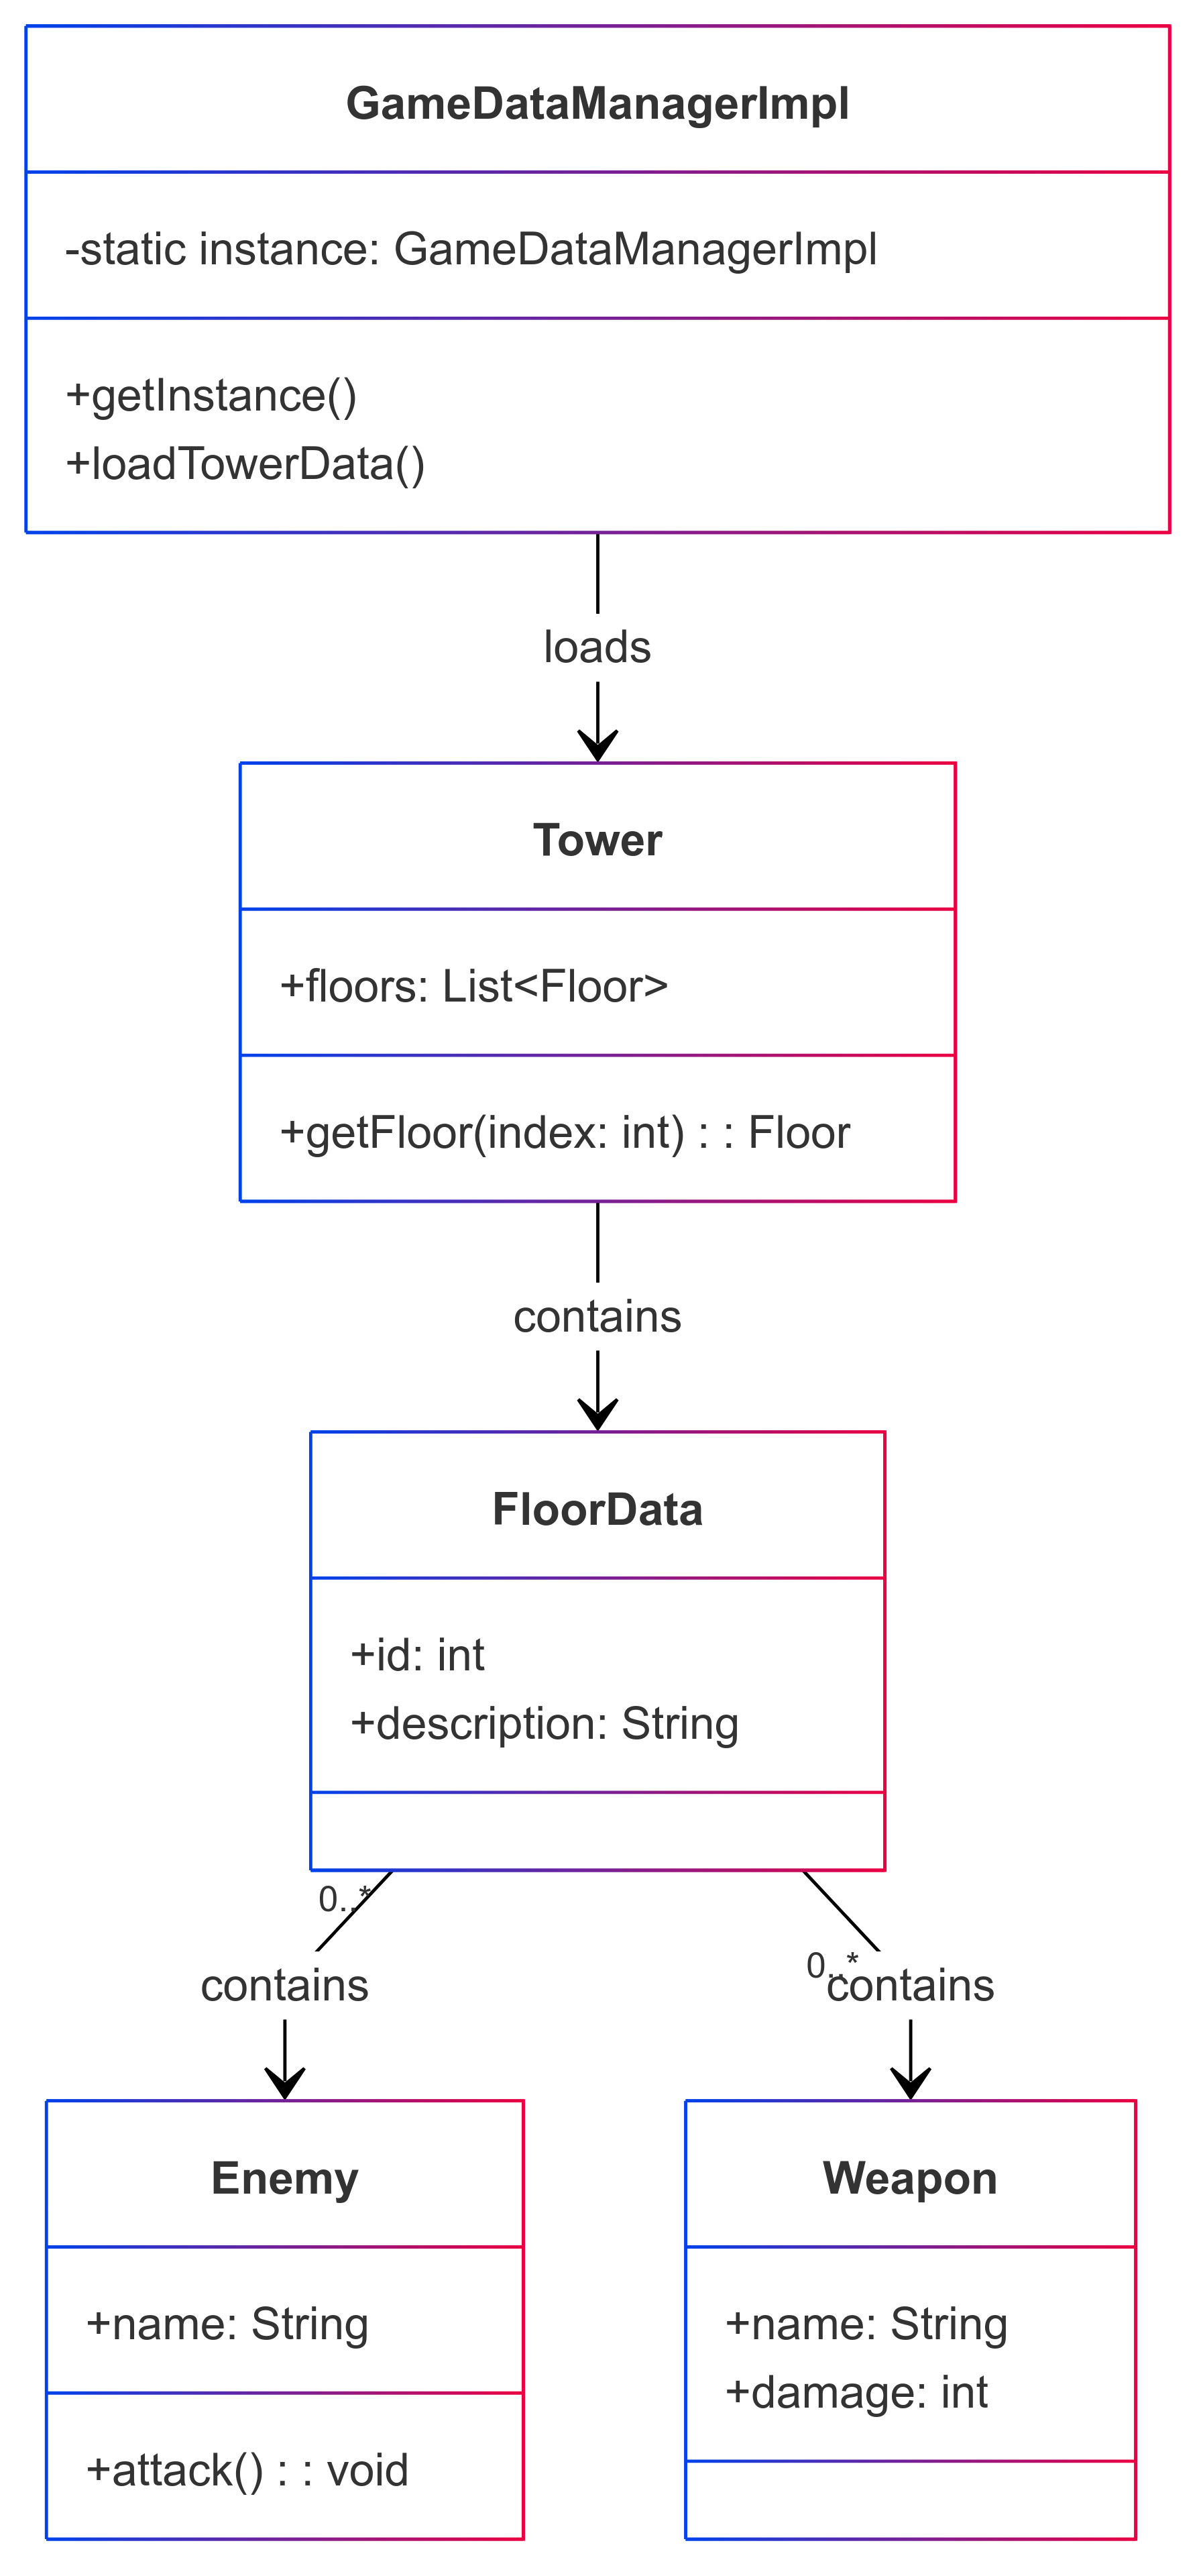
\includegraphics[scale=0.08]{img/GameDataManagerUML.png}
	\caption{GameDataManagerImpl as Singleton and its relations.}
\end{figure}

\subsubsection{Sistema di Modding}

\paragraph{Problema} Il gioco deve permettere agli utenti di creare e importare torri personalizzate (mod) sia da cartelle che da file ZIP, gestendo validazione, conflitti di nomi e isolamento tra mod.

\paragraph{Soluzione} Ho considerato due possibili architetture:

\begin{enumerate}
    \item Un sistema event-based con chiamate asincrone per l'importazione
    \item Un'architettura MVC con Observer pattern per la sincronizzazione UI
\end{enumerate}
Ho scelto la seconda opzione perché offre una separazione più chiara delle responsabilità e una gestione più prevedibile dello stato. Il pattern Observer è stato preferito a un sistema di callback perché permette di aggiungere facilmente nuovi observer senza modificare il codice esistente.

Ho implementato anche il pattern Strategy per l'importazione, permettendo di aggiungere facilmente nuovi formati di mod oltre a ZIP e cartelle.

Schema UML:
\begin{figure}[H]
	\centering
	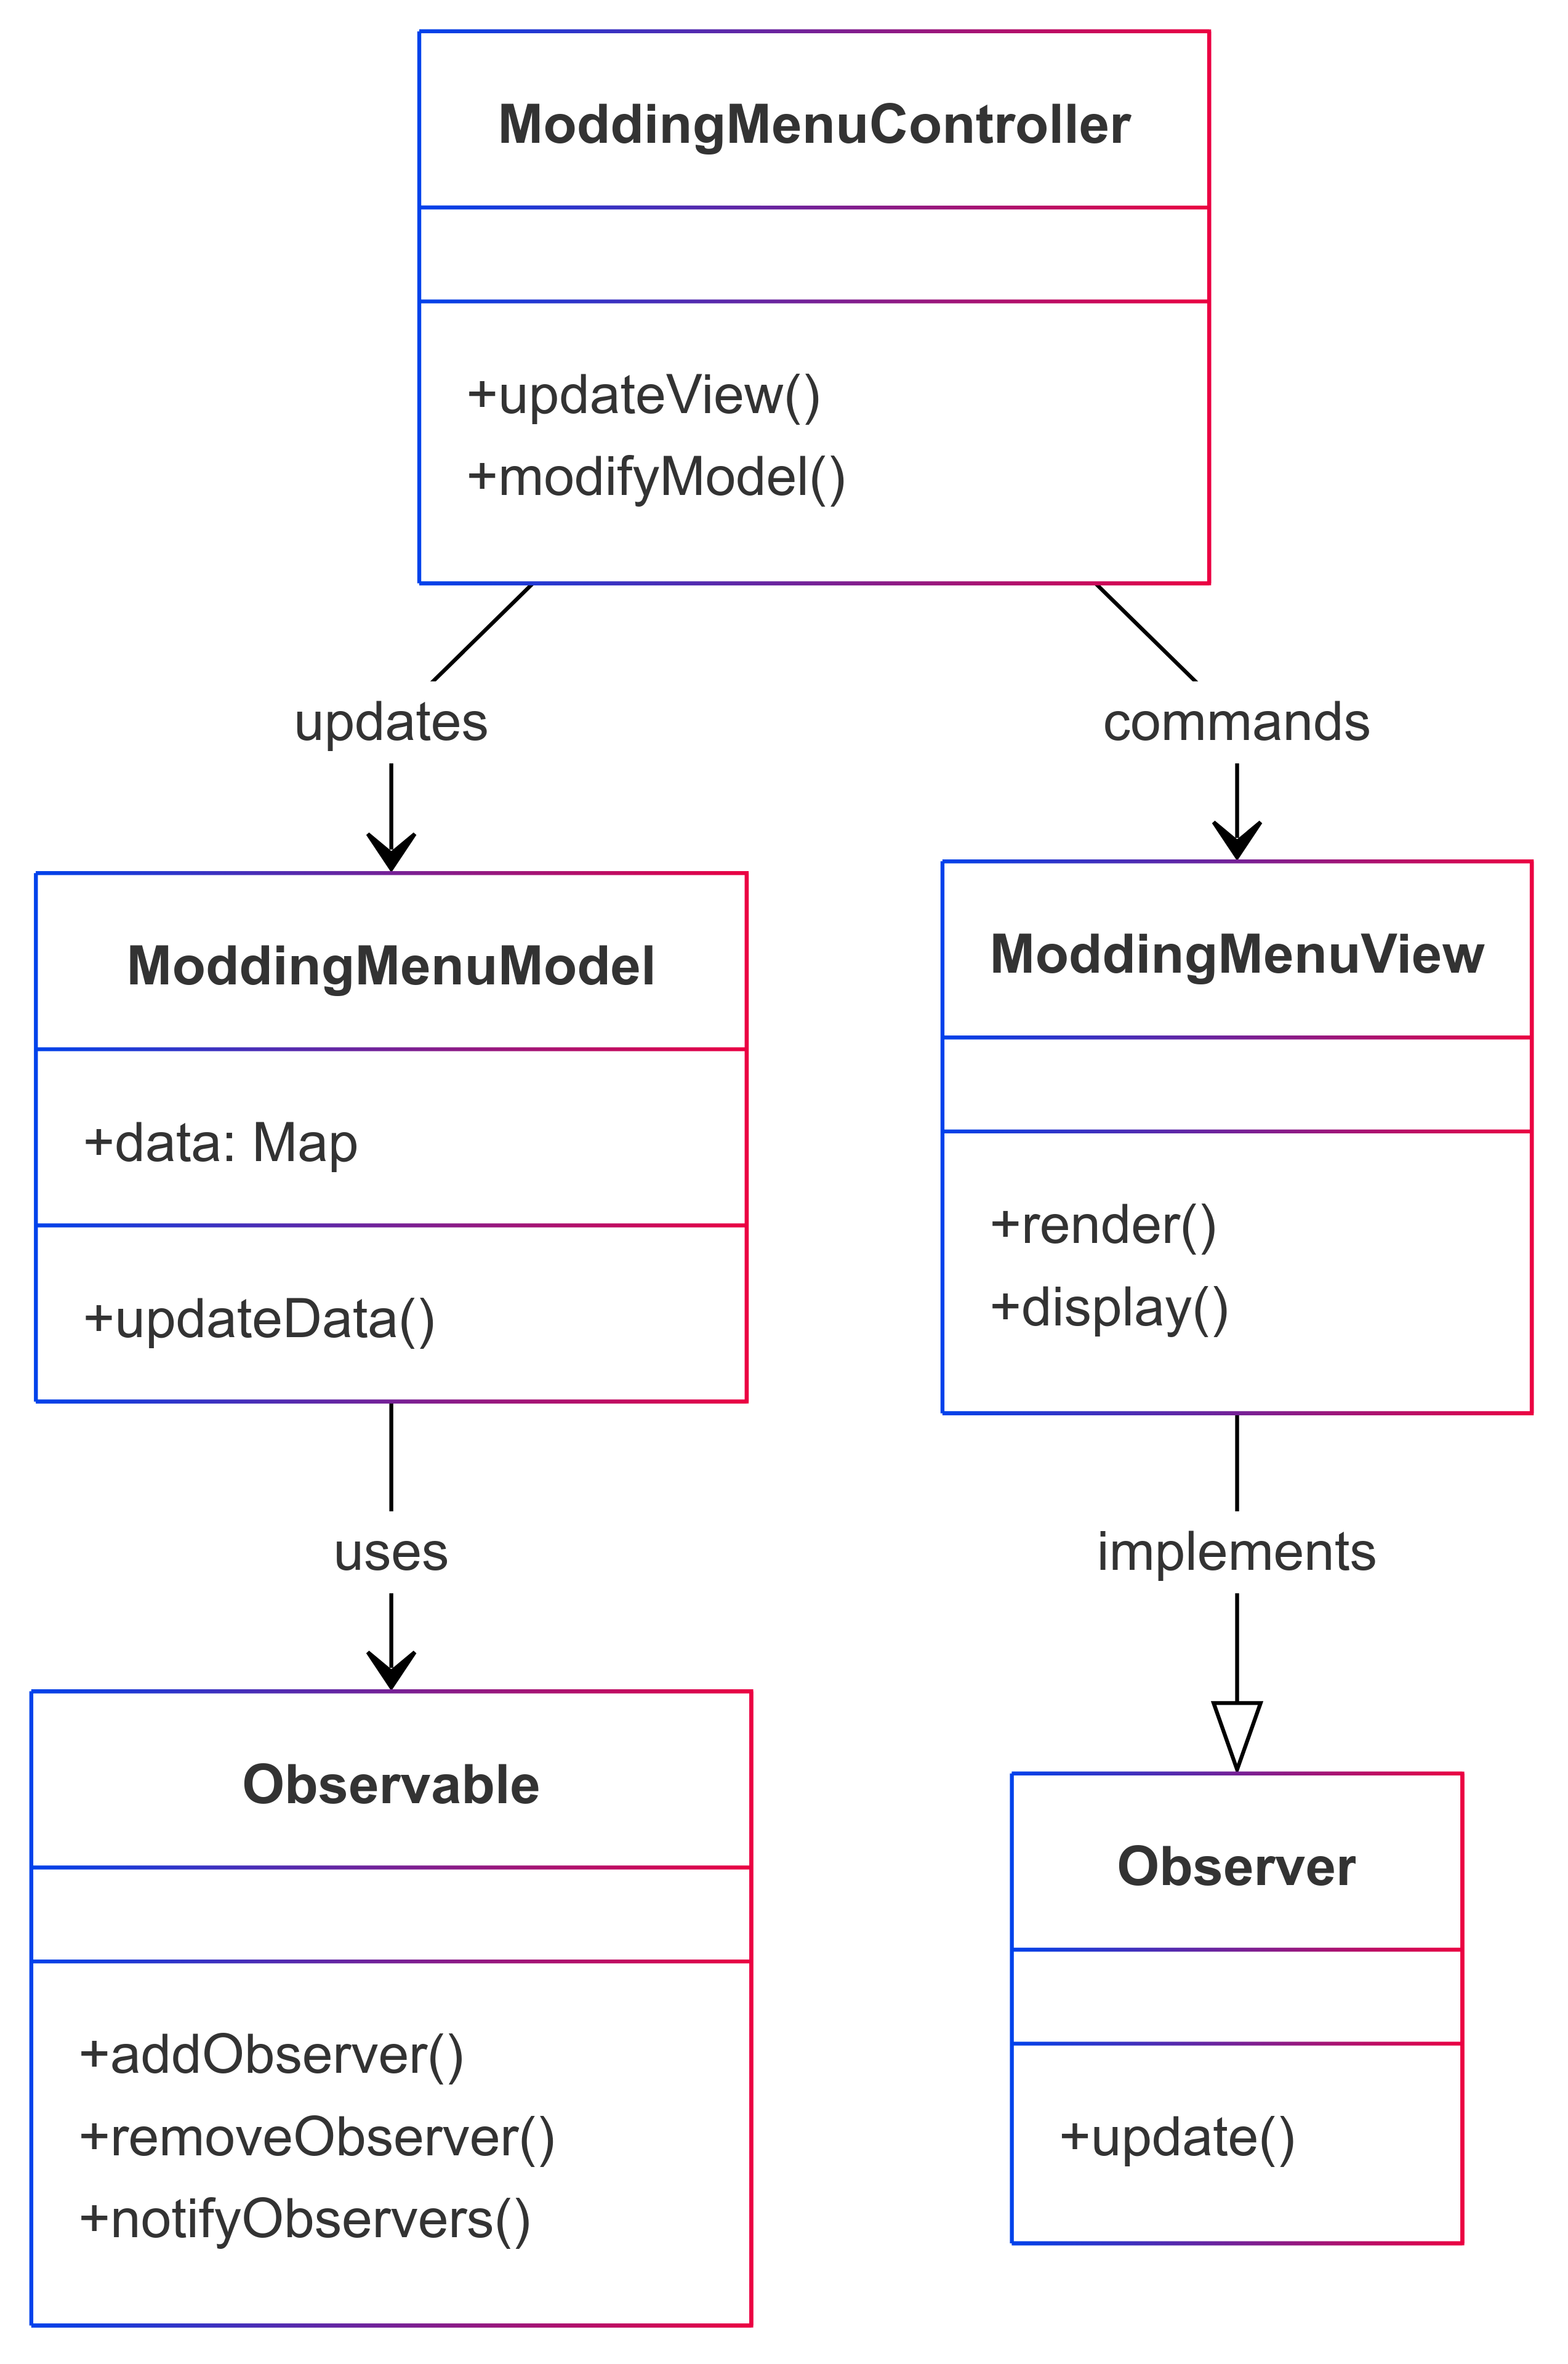
\includegraphics[scale=0.08]{img/ModdingMenuUML.png}
	\caption{Modding Menu UML: MVC and Observer pattern overview.}
\end{figure}

\subsubsection{Gestione dello Spawn System}

\paragraph{Problema} Il sistema deve generare contenuti procedurali bilanciati rispettando vincoli di livello e configurazioni di spawn.

\paragraph{Soluzione} Ho valutato due approcci:
\begin{enumerate}
	\item Generazione puramente casuale con post-validazione
	\item Sistema template-based con strategie di Generazione
\end{enumerate}

Ho scelto il secondo approccio implementando un Template Method in SpawnManagerImpl che standardizza il processo di generazione permettendo variazioni nel comportamento specifico. Questo pattern è stato preferito a una soluzione più flessibile ma potenzialmente caotica basata su eventi.
Il metodo template definisce tre fasi:
\begin{enumerate}
	\item Selezione del tipo di piano (template method).
	\item Generazione delle stanze (hook method).
	\item Popolamento delle stanze (hook method).
\end{enumerate}

\subsection{Mularoni}

\subsubsection{Cambio vista}

\begin{figure}[H]
\centering{}
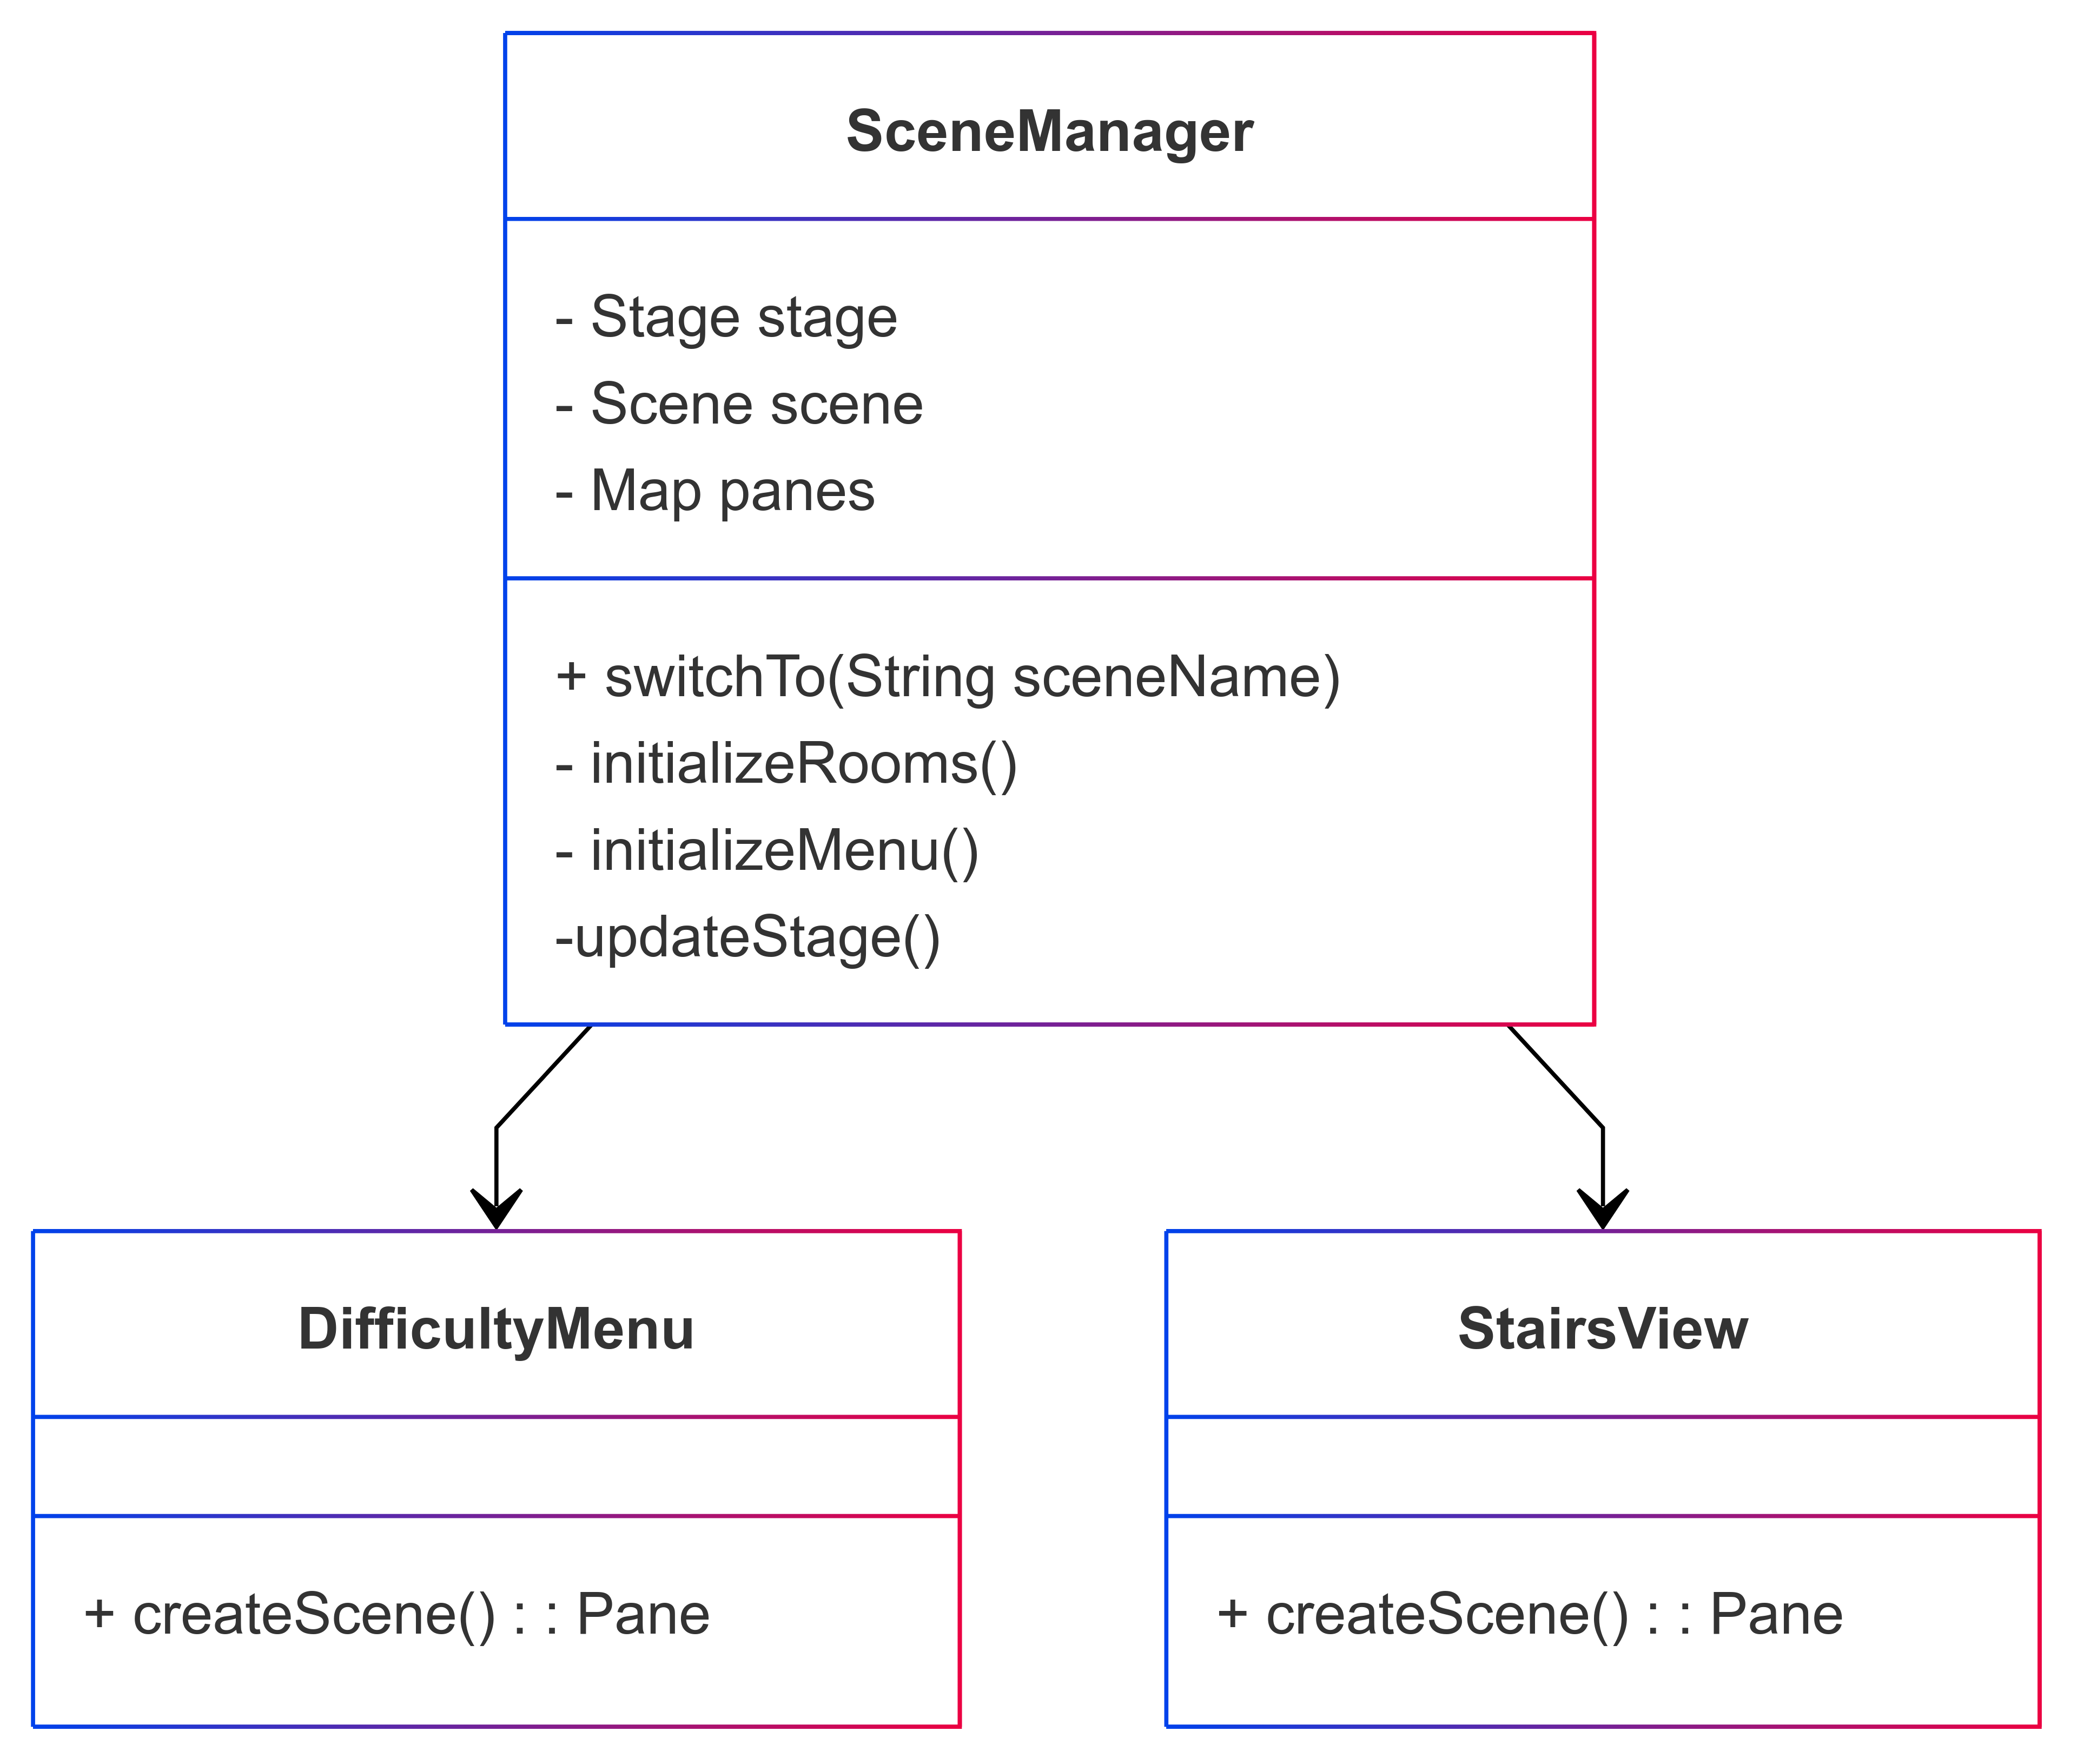
\includegraphics[width=\textwidth]{img/scenemanager.png}
\caption{Rappresentazione UML del pattern Factory per la gestione delle viste (esempio con 2 viste)}
\label{img:factory}
\end{figure}

\paragraph{Problema} Il gioco ha diverse viste, una per ogni situazione (Menu iniziale, vista sulle stanze, stanze singole ecc...),
%
è necessario gestire la visualizzazione in un modo coerente.

\paragraph{Soluzione} Il sistema per la gestione delle viste utilizza il \textit{pattern Factory}, come da
\Cref{img:factory}: le classi che implementano le viste \texttt{NomevistaView} una volta create, vengono inserite nel mapping
%
interno di \texttt{SceneManager} il quale si occupa di: 
\begin{itemize}
	\item All'avvio del gioco: inizializzare le viste relative alle schermate inziali.
	\item Dopo il caricamento della torre: inizializzare le viste degli elementi di gioco.
	\item Quando si chiama \texttt{switchTo}: caricare il nuovo Pane nella scena e visualizzarlo.
\end{itemize}
Questa soluzione permette in ogni parte della view, richiamando \texttt{switchTo} di passare alla view successiva passando il nome di essa,
%
permettendo una certa flessibilità nella creazione e linking di eventuali nuove viste.

\subsubsection{Stanze del gioco}

\begin{figure}[H]
\centering{}
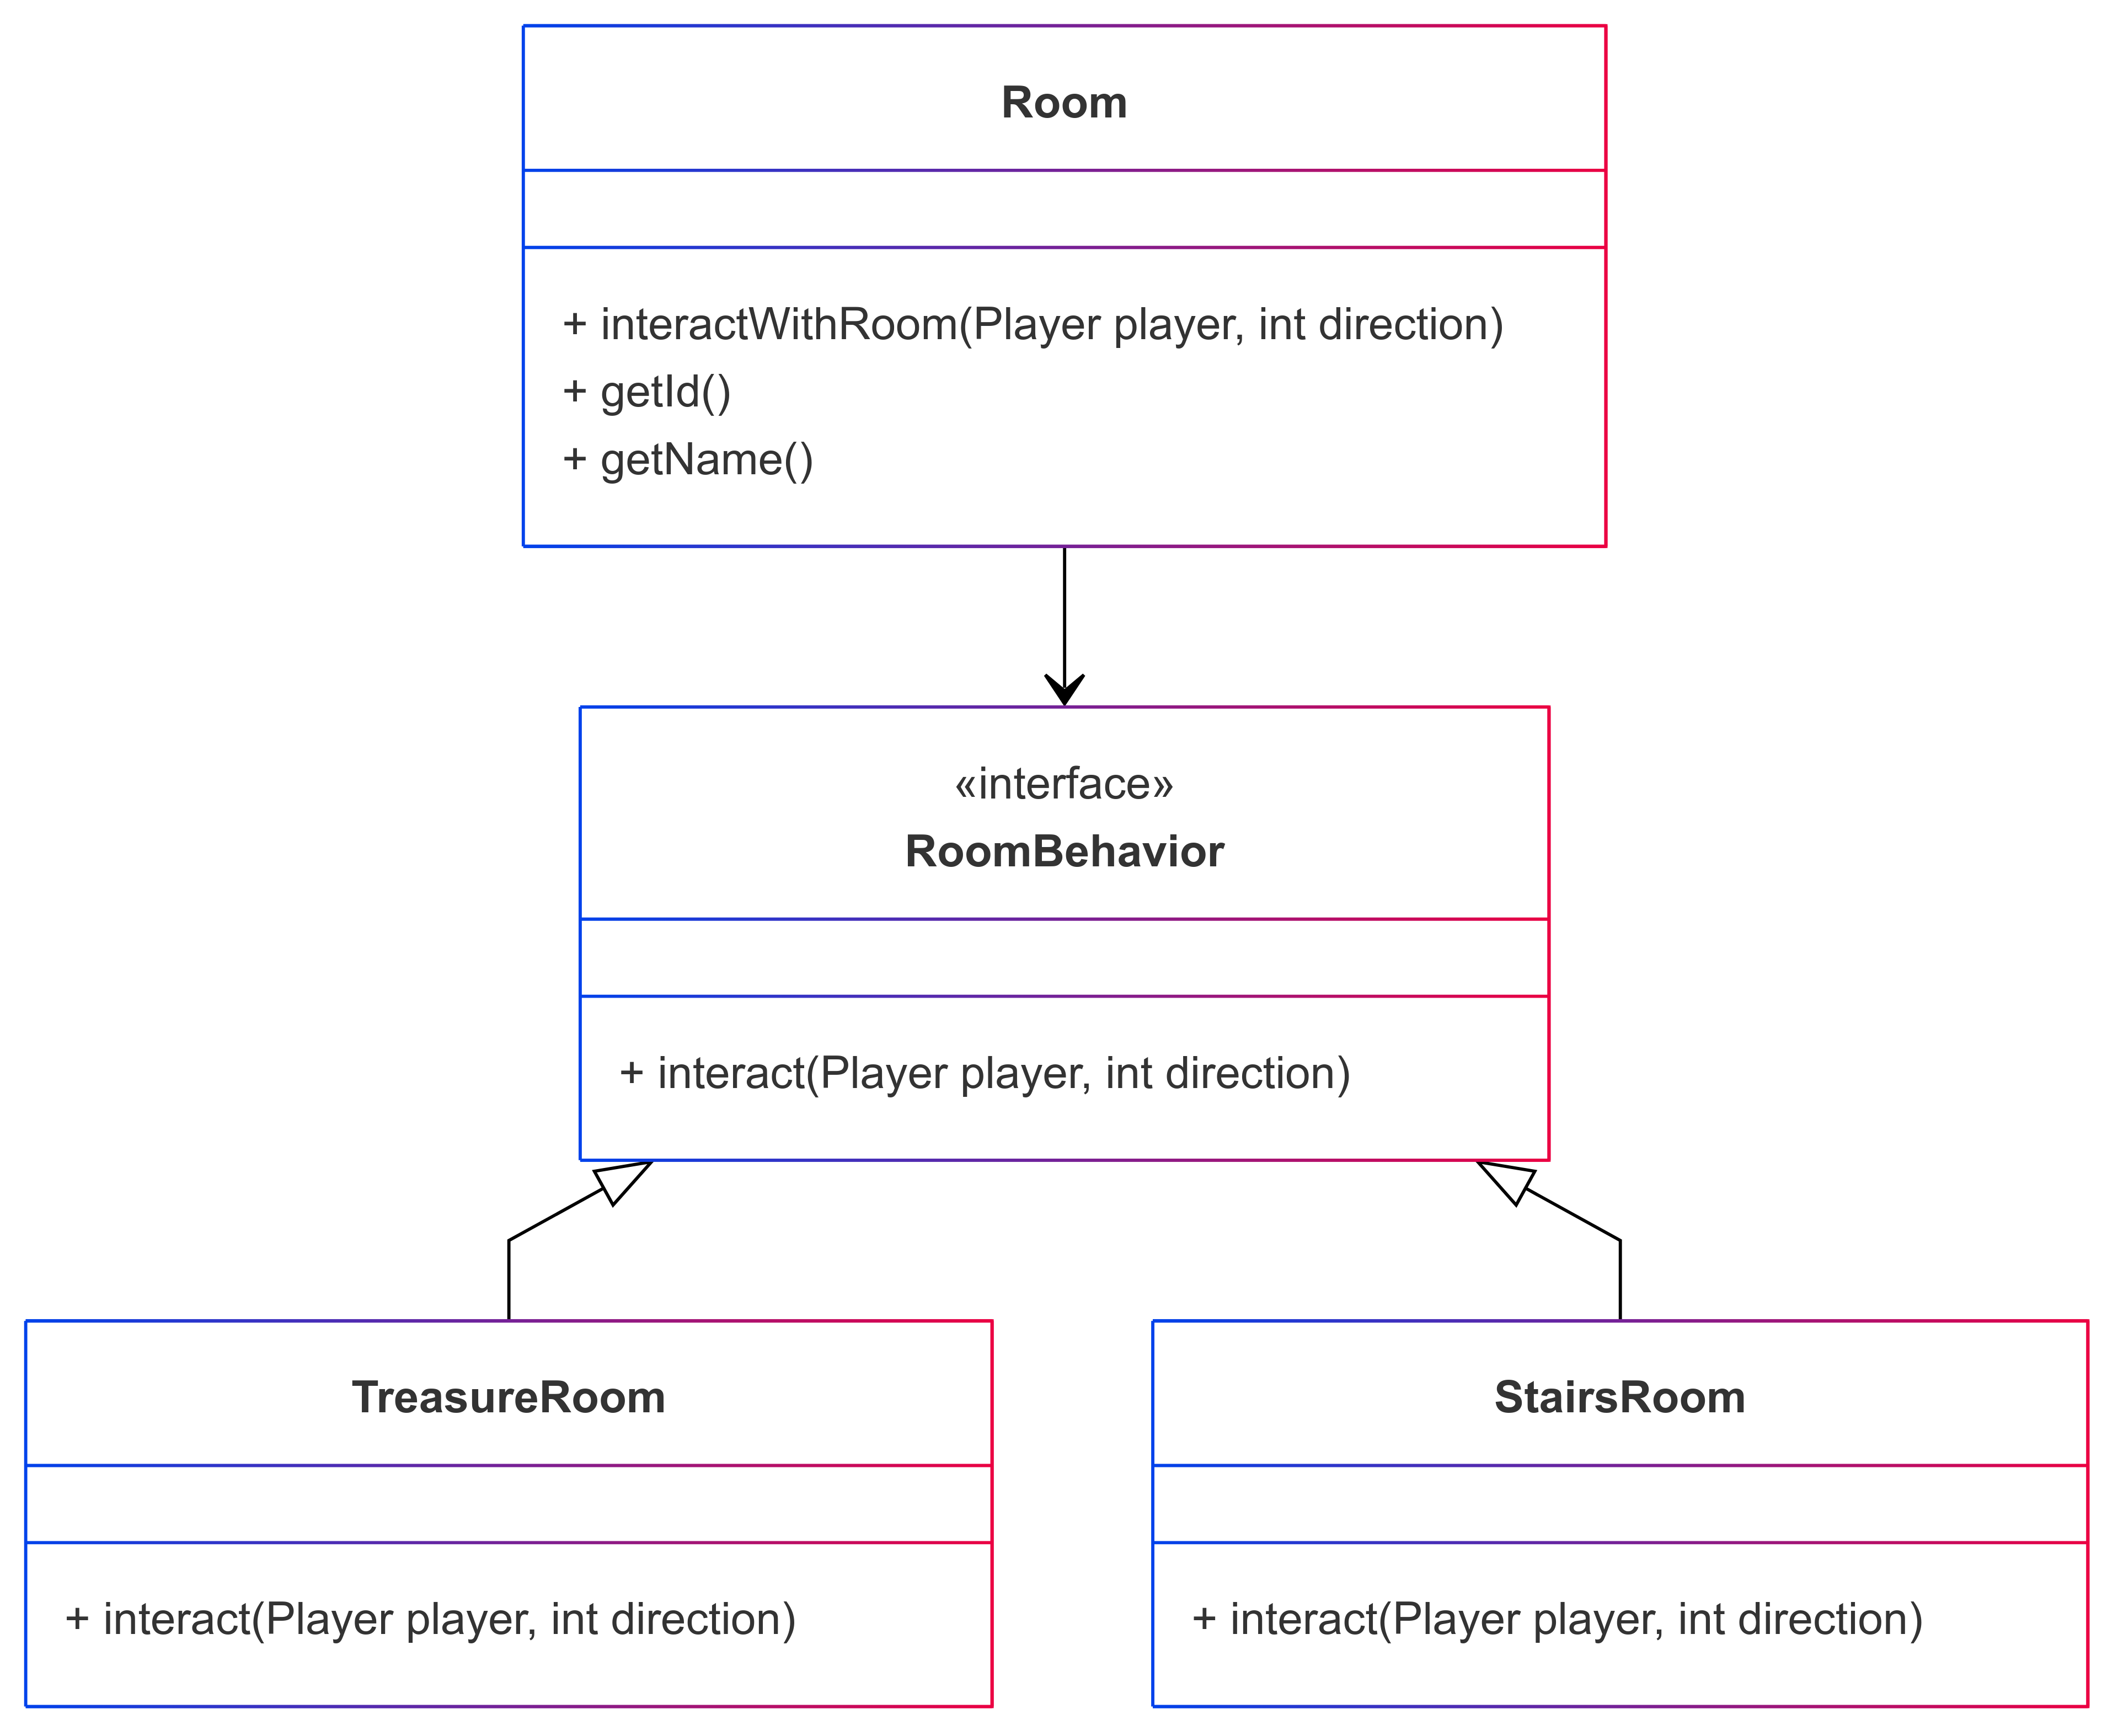
\includegraphics[width=\textwidth]{img/behavior.png}
\caption{Rappresentazione UML del pattern Strategy per le stanze del gioco}
\label{img:rooms}
\end{figure}

\paragraph{Problema} Temple Tower ha più stanze, ognuna con un contenuto differente.

\paragraph{Soluzione} Il sistema per la modellazione delle stanze utilizza il \textit{pattern Strategy}, come da
\Cref{img:rooms}: le implementazioni di \texttt{RoomBehavior} possono essere modificate, e a seconda di cosa si inserisce nel metodo
%
\texttt{interact()}, il giocatore subirà o lancierà (a seconda di \texttt{direction}) delle azione da/alla stanza.
%
Per esempio un metodo interact dentro Trap toglierà punti vita al Player, mentre la stanza Stairs cambierà il piano di quest'ultimo.
%
Questo pattern permette di ampliare i tipi possibili di stanze richiedendo poche modifiche all'interno del codice già esistente. 

\chapter{Sviluppo}
\section{Testing automatizzato}
Per il testing generale di Temple Tower è stato utilizzata la suite JUnit per il testing automatizzato.
\subsection*{Controller}
Sono state testate nel controller, tutte le classi che interagiscono tramite esso, nella view.

\begin{itemize}
 \item Giocatore: vita, cambio stanza e armi.
 \item Nemico: vita e attacchi.
 \item Cambio piano.
 \item Boss finale: sistema di decisione sull'arrivo alla stanza del boss finale.
\end{itemize}

\section{Note di sviluppo}

Questa sezione, come quella riguardante il design dettagliato va svolta \textbf{singolarmente da ogni membro del gruppo}.
%
Nella prima parte, ciascuno dovrà mostrare degli esempi di codice particolarmente ben realizzati,
che dimostrino proefficienza con funzionalità avanzate del linguaggio e capacità di spingersi oltre le librerie mostrate a lezione.

\begin{itemize}
	\item \textbf{Elencare} (fare un semplice elenco per punti, non un testo!) le feature \textit{avanzate} del linguaggio e dell'ecosistema Java che sono state
utilizzate. Le feature di interesse sono:
	\begin{itemize}
		\item Progettazione con generici, ad esempio costruzione di nuovi tipi generici, e uso di generici bounded.
		L'uso di classi generiche di libreria non è considerato avanzato.
		\item Uso di lambda expressions
		\item Uso di \texttt{Stream}, di \texttt{Optional} o di altri costrutti funzionali
		\item Uso di reflection
		\item Definizione ed uso di nuove annotazioni
		\item Uso del Java Platform Module System
		\item Uso di parti della libreria JDK non spiegate a lezione (networking, compressione, parsing XML, eccetera...)
		\item Uso di librerie di terze parti (incluso JavaFX): Google Guava, Apache Commons...
	\end{itemize}
	\item Si faccia molta attenzione a non scrivere banalità, elencando qui features di tipo ``core'', come le eccezioni, le enumerazioni, o le inner class: nessuna di queste è considerata avanzata.
	\item Per ogni feature avanzata, mostrata, includere:
	\begin{itemize}
		\item Nome della feature
		\item Permalink GitHub al punto nel codice in cui è stata utilizzata
	\end{itemize}
\end{itemize}

In questa sezione, \textit{dopo l'elenco},
vanno menzionati ed attributi con precisione eventuali pezzi di codice ``riadattati'' (o scopiazzati...) da Internet o da altri progetti,
pratica che tolleriamo ma che non raccomandiamo.
%
Si rammenta agli studenti che non è consentito partire da progetti esistenti e procedere per modifiche successive.
%
Si ricorda anche che i docenti hanno in mano strumenti antiplagio piuttosto raffinati e che ``capiscono'' il codice e la storia delle modifiche del progetto,
per cui tecniche banali come cambiare nomi (di classi, metodi, campi, parametri, o variabili locali),
aggiungere o togliere commenti,
oppure riordinare i membri di una classe vengono individuate senza problemi.
%
Le regole del progetto spiegano in dettaglio l'approccio dei docenti verso atti gravi come il plagiarismo.

I pattern di design \textbf{non} vanno messi qui.
%
L'uso di pattern di design (come suggerisce il nome) è un aspetto avanzato di design, non di implementazione,
e non va in questa sezione.

\subsection*{Elementi positivi}

\begin{itemize}
	\item Si elencano gli aspetti avanzati di linguaggio che sono stati impiegati
	\item Si elencano le librerie che sono state utilizzate
	\item Per ciascun elemento, si fornisce un permalink
	\item Ogni permalink fa riferimento ad uno snippet di codice scritto dall'autore della sezione (i docenti verificheranno usando \texttt{git blame})
	\item Se si è utilizzato un particolare algoritmo, se ne cita la fonte originale.
	Ad esempio, se si è usato Mersenne Twister per la generazione di numeri pseudo-random, si cita \cite{mersenne}.
	\item Si identificano parti di codice prese da altri progetti, dal web, o comunque scritte in forma originale da altre persone.
	In tal senso, si ricorda che agli ingegneri non è richiesto di re-inventare la ruota continuamente:
	se si cita debitamente la sorgente è tollerato fare uso di di snippet di codice open source per risolvere velocemente problemi non banali.
	Nel caso in cui si usino snippet di codice di qualità discutibile,
	oltre a menzionarne l'autore originale si invitano gli studenti ad adeguare tali parti di codice agli standard e allo stile del progetto.
	Contestualmente, si fa presente che è largamente meglio fare uso di una libreria che copiarsi pezzi di codice:
	qualora vi sia scelta (e tipicamente c'è), si preferisca la prima via.
\end{itemize}

\subsection*{Elementi negativi}
\begin{itemize}
	\item Si elencano feature core del linguaggio invece di quelle segnalate. Esempi di feature core da non menzionare sono:
    \begin{itemize}
        \item eccezioni;
        \item classi innestate;
        \item enumerazioni;
        \item interfacce.
    \end{itemize}
	\item Si elencano applicazioni di terze parti (peggio se per usarle occorre licenza, e lo studente ne è sprovvisto) che non c'entrano nulla con lo sviluppo, ad esempio:
    \begin{itemize}
        \item Editor di grafica vettoriale come Inkscape o Adobe Illustrator;
        \item Editor di grafica scalare come GIMP o Adobe Photoshop;
        \item Editor di audio come Audacity;
        \item Strumenti di design dell'interfaccia grafica come SceneBuilder: il codice è in ogni caso inteso come sviluppato da voi.
    \end{itemize}
	\item Si descrivono aspetti di scarsa rilevanza, o si scende in dettagli inutili.
	\item Sono presenti parti di codice sviluppate originalmente da altri che non vengono debitamente segnalate.
	In tal senso, si ricorda agli studenti che i docenti hanno accesso a tutti i progetti degli anni passati,
	a Stack Overflow,
	ai principali blog di sviluppatori ed esperti Java,
	ai blog dedicati allo sviluppo di soluzioni e applicazioni
	(inclusi blog dedicati ad Android e allo sviluppo di videogame),
	nonché ai vari GitHub, GitLab, e Bitbucket.
	Conseguentemente, è \emph{molto} conveniente \emph{citare} una fonte ed usarla invece di tentare di spacciare per proprio il lavoro di altri.
	\item Si elencano design pattern
\end{itemize}

\subsection{Vignali}
\subsubsection{Utilizzo della libreria gson}
Utilizzato principalmente in GameDataManager per l'importazione e il caricamento delle torri: \href{https://google.com}{permalink}/ 
\subsubsection{Utilizzo della libreria JavaFX}
Utilizato All'interno di ModdingMenuView insieme a codice CSS: \href{https://google.com}{permalink}/ 
\subsubsection{Utilizzo della libreria SL4J}
Utilizzato per la gestione dei log principalemente nei test ma anche in giro per il codice: \href{https://google.com}{permalink}/ 
\subsubsection{Utilizzo della libreria Apache Commons IO}
Utilizzato per la gestione dei file insime alla java util per l'importazione dei file: \href{https://google.com}{permalink}/ 
\subsubsection{Utilizzo della libreria Java util zip}
Utilizzato per la decompressione dei file: \href{https://google.com}{permalink} 
\subsubsection{Utilizzo di stream e lambda expressions}
Utilizzato in diverse parti qui un esempio: \href{https://google.com}{permalink} 
\subsubsection{Utilizzo di Optional}
Utilizzato in diverse parti qui un esempio: \href{https://google.com}{permalink} 

\subsection{Mularoni}
\subsubsection{Utilizzo di \texttt{Stream} e lambda expressions} - Esempio: \href{https://google.com}{permalink}/ 
\subsubsection{Utilizzo di \texttt{Threading e Task} in Javafx per prevenire race condition} - Esempio: \href{https://google.com}{permalink}/ 
\subsubsection{Utilizzo della libreria SLF4J} - Esempio: \href{https://google.com}{permalink}/ 
\subsubsection{Cerchi con javafx} - Fonte: \href{https://stackoverflow.com/questions/70876114/click-to-draw-a-shape-circle}{Stackoverflow}/ 
\subsubsection{Immagini con javafx} - Fonte: \href{https://stackoverflow.com/questions/52229984/javafx-imageview-actions}{Stackoverflow}/ 
\subsubsection{Uso di Platform.runLater()} - Fonte: \href{https://stackoverflow.com/questions/13784333/platform-runlater-and-task-in-javafx}{Stackoverflow}/ 

\subsection{Montanari}
\subsubsection{Uso di SLF4J per il logging}
Il progetto utilizza il framework SLF4J per la gestione dei log. Questo consente un monitoraggio efficace degli eventi di gioco.\newline
Esempio di codice:
\begin{verbatim}
private static final Logger LOGGER = LoggerFactory.getLogger(GameControllerImpl.class);
\end{verbatim}
\href{https://github.com/}{Link al codice su GitHub}

\subsubsection{Uso di Lambda Expressions}
Per la gestione degli eventi, il codice utilizza espressioni lambda che migliorano la leggibilità e riducono la verbosità.\newline
Esempio:
\begin{verbatim}
attackBt.setOnAction(e -> this.performAttack());
\end{verbatim}
\href{https://github.com/}{Link al codice su GitHub}

\subsubsection{Gestione del multithreading con Platform.runLater}
JavaFX richiede che gli aggiornamenti dell'interfaccia avvengano nel thread principale. Platform.runLater viene utilizzato per garantire che le modifiche alla UI siano eseguite in modo sicuro.\newline
Esempio:
\begin{verbatim}
Platform.runLater(() -> playerHpBar.setProgress(newHealth / (double) maxHealth));
\end{verbatim}
\href{https://github.com/}{Link al codice su GitHub}

\subsubsection{Utilizzo di Timeline e KeyFrame per le animazioni}
Il codice implementa animazioni utilizzando Timeline e KeyFrame, creando effetti visivi per gli attacchi e la riduzione della vita dei personaggi.\newline
Esempio:
\begin{verbatim}
Timeline attackAnimation = new Timeline(
new KeyFrame(Duration.seconds(0.5), e -> enemyHpBar.setProgress(newEnemyHp / (double) maxEnemyHp))
);
attackAnimation.play();
\end{verbatim}
\href{https://github.com/}{Link al codice su GitHub}

\subsubsection{Utilizzo di JavaFX Scene Graph}
La costruzione dell'interfaccia utente avviene attraverso l'uso di StackPane, HBox, VBox e BorderPane.\newline
\href{https://github.com/}{Link al codice su GitHub}
\subsection{Cobo}

\subsection{Esempio}

\subsubsection{Utilizzo della libreria SLF4J}

Utilizzata in vari punti.
Un esempio è \url{https://github.com/AlchemistSimulator/Alchemist/blob/5c17f8b76920c78d955d478864ac1f11508ed9ad/alchemist-swingui/src/main/java/it/unibo/alchemist/boundary/swingui/effect/impl/EffectBuilder.java#L49}

\subsubsection{Utilizzo di \texttt{LoadingCache} dalla libreria Google Guava}

Permalink: \url{https://github.com/AlchemistSimulator/Alchemist/blob/d8a1799027d7d685569e15316a32e6394632ce71/alchemist-incarnation-protelis/src/main/java/it/unibo/alchemist/protelis/AlchemistExecutionContext.java#L141-L143}

\subsubsection{Utilizzo di \texttt{Stream} e lambda expressions}

Usate pervasivamente. Il seguente è un singolo esempio.
Permalink: \url{https://github.com/AlchemistSimulator/Alchemist/blob/d8a1799027d7d685569e15316a32e6394632ce71/alchemist-incarnation-protelis/src/main/java/it/unibo/alchemist/model/ProtelisIncarnation.java#L98-L120}

\subsubsection{Scrittura di metodo generico con parametri contravarianti}

Permalink: \url{https://github.com/AlchemistSimulator/Alchemist/blob/d8a1799027d7d685569e15316a32e6394632ce71/alchemist-incarnation-protelis/src/main/java/it/unibo/alchemist/protelis/AlchemistExecutionContext.java#L141-L143}

\subsubsection{Protezione da corse critiche usando \texttt{Semaphore}}

Permalink: \url{https://github.com/AlchemistSimulator/Alchemist/blob/d8a1799027d7d685569e15316a32e6394632ce71/alchemist-incarnation-protelis/src/main/java/it/unibo/alchemist/model/ProtelisIncarnation.java#L388-L440}


\chapter{Commenti finali}

\section{Vignali}
Penso che la parte scritta da me sia stata fatta al meglio per il tempo a disposizione, e il fatto di aver passato molto tempo iniziale a 
%
pensare su come far funzionare la questione dei Json è servita, alcuni dati che inizialmente avevo pensato di inserire nella mia parte che era principalmente la struttura dati li ho dovuti
%
rimuovere per non appesantire troppo il lavoro ai miei compagni, mentre alcuni non sono stati utilizzati anche se inseriti,
%
tutto sommato sono soddisfatto della mia parte e del mio codice, la feature più grande che ho dovuto rimuovere per mancanza di tempo è
%
la creazione tramite interfaccia di torri personalizzate, probabilmente sarebbero servite 15-20 ore extra per implemtarla e sarebbe stato molto interessante svilupparla quindi potrebbe essere una dei lavori futuri
\section{Mularoni}
Considerando il tempo a disposizione e gli impegni derivanti da lavoro e altri esami, reputo questo progetto "accettabile" ma con un grande potenziale inespresso,
%
dovuto sia alla scarsa divisibilità del progetto a livello di idea (è difficile che tutti lavorino a compartimenti stagni) che di organizzazione generale.
\section{Montanari}
Durante lo sviluppo del progetto, mi sono occupato principalmente del sistema di combattimento, della creazione delle varie view di gioco e del controller in modo da far comunicare tutte le classi tra di loro. Ritengo che i miei punti di forza siano stati la capacità di problem-solving, la scrittura di codice efficiente e la collaborazione con il team. Tuttavia, ho riscontrato alcune difficoltà, in particolare nella gestione del tempo e nel debugging di problemi complessi.

\subsubsection{Ruolo all'interno del gruppo}
All'interno del team, il mio ruolo è stato quello di sviluppatore principale per il sistema di combattimento e le interfacce di gioco, oltre a occuparmi della logica di comunicazione tra le classi. Ho contribuito a garantire che tutte le componenti funzionassero correttamente insieme, cercando di mantenere un buon livello di collaborazione con gli altri membri.

\subsubsection{Lavori futuri}
Se il progetto dovesse essere portato avanti, credo che si potrebbe migliorare in diverse direzioni. In particolare, suggerirei di ottimizzare le prestazioni del sistema di combattimento, migliorare l'interfaccia utente e aggiungere nuove funzionalità per rendere il gioco più coinvolgente. Inoltre, potrebbe essere utile impiegare il progetto come base per un gioco più ampio o come portfolio personale per dimostrare le competenze acquisite.

Nel complesso, questa esperienza mi ha permesso di migliorare le mie competenze in programmazione, gestione delle comunicazioni tra classi e sviluppo di interfacce di gioco, e sono soddisfatto dei progressi fatti.

\section{Cobo}
Mi sono occupato della gestione dell’audio e dell’integrazione del sistema musicale nel progetto. Ho implementato il controllo della musica di sottofondo, il sistema di regolazione del volume e la gestione della riproduzione attraverso il pattern Singleton. Inoltre mi sono occupato della gestione delle scene e dell’interfaccia utente, implementando i menu, ad esempio quello delle impostazioni che ha pulsanti per il controllo del volume e per la navigazione tra schermate.

\subsubsection{Punti di forza}
Utilizzo avanzato di Java Sound API per il controllo dell’audio.
Implementazione del pattern Singleton con doppia verifica per garantire efficienza e sicurezza.
Utilizzo di JavaFX per un'interfaccia grafica responsive e dinamica.
Creazione di pulsanti grafici con immagini per un’interfaccia più intuitiva.
Organizzazione chiara del codice, rendendo i menu facilmente estendibili.
\subsubsection{Punti di debolezza}
La gestione del volume potrebbe essere migliorata con un'interfaccia utente più intuitiva.
Alcune transizioni tra scene potrebbero essere più fluide e animate.
L’aspetto visivo del menu potrebbe essere più curato con CSS.
\subsubsection{Lavori futuri}
Se il progetto venisse portato avanti, si potrebbe migliorare il sistema audio offrendo un maggiore controllo e una qualità audio migliore. Inoltre si potrebbe aggiungere un file di configurazione per memorizzare le preferenze dell’utente e un design UI più accattivante con animazioni e transizioni fluide.
Durante il corso mi sono trovato molto bene con i docenti, sia per la chiarezza delle spiegazioni sia per l’efficacia dei metodi di insegnamento adottati. Il materiale fornito e l’approccio didattico hanno reso l’apprendimento strutturato e accessibile, facilitando la comprensione anche di concetti avanzati.
\appendix
\chapter{Guida utente}

Abbiamo cercato di rendere l'applicazione il più facile possibile da utilizzare.
%
Una volta avviata all'utente basterà cliccare il bottone su schermo per arrivare al menu principale,
%
a questo punto serve importare una qualunque torre tramite il Modding Menu, e selezionarla per poter giocare, la tower si troverà nella repository
%
oppure può essere scaricata da questo link \href{https://google.com}{(Tower Download)}. La tower può essere selezionata in una qualunque posizione
%
all'interno del proprio pc, una volta selezionata si può iniziare a giocare, cliccando il bottone centrale, si consiglia di utilizzare la difficoltà facile per motivi di testing,
%
a questo punto per giocare si può girare a destra oppure sinistra con i due bottoni in basso e cliccando il bottone centrale
%
si può entrare in una delle stanze, una volta entrato basterà seguire le istruzioni su schermo;

\chapter{Esercitazioni di laboratorio}

\subsection{mattia.mularoni@studio.unibo.it}

\begin{itemize}
\item Laboratorio 07: \url{https://virtuale.unibo.it/mod/forum/discuss.php?d=177162#p246190}
 \item Laboratorio 08: \url{https://virtuale.unibo.it/mod/forum/discuss.php?d=178723#p247234}
 \item Laboratorio 09: \url{https://virtuale.unibo.it/mod/forum/discuss.php?d=179154#p247924}
 \item Laboratorio 10: \url{https://virtuale.unibo.it/mod/forum/discuss.php?d=180101#p249553}
 \item Laboratorio 04: \url{https://virtuale.unibo.it/mod/forum/discuss.php?d=12345#p123456}
 \item Laboratorio 06: \url{https://virtuale.unibo.it/mod/forum/discuss.php?d=22222#p222222}
 \item Laboratorio 09: \url{https://virtuale.unibo.it/mod/forum/discuss.php?d=99999#p999999}
\end{itemize}

\subsection{davide.vignali4@studio.unibo.it}

\begin{itemize}
 \item Laboratorio 09: \url{https://virtuale.unibo.it/mod/forum/discuss.php?d=179154#p248027}
\end{itemize}

\subsection{nicolas.montanari3@studio.unibo.it}

\begin{itemize}
 \item Laboratorio 09: \url{https://virtuale.unibo.it/mod/forum/discuss.php?d=179154}
 \item Laboratorio 10: \url{https://virtuale.unibo.it/mod/forum/discuss.php?d=180101}
\end{itemize}


\bibliographystyle{alpha}
\bibliography{13-template}

\end{document}
